\chapter{Подготовка верификационных задач}

В данной главе описан процесс подготовки верификационных задач, в основе которого лежат новые методы автоматизированной декомпозиции Си-программ на модули и синтеза для них моделей окружения.

\section{Программный интерфейс модулей Си-программ}
Процесс генерации верификационных задач предполагает выполнение декомпозиции программной системы на языке программирования Си на модули, для каждого из которых в зависимости от его программного интерфейса выполняется подготовка соответствующих моделей окружения и требований.
Прежде чем изложить новые методы, рассмотрим что из себя представляет программный интерфейс таких модулей.

Модулем программы называется один или несколько Си-файлов с исходным кодом программы.
Построенная на основе модуля программы верификационная задача содержит препроцессированный исходный код данных файлов.
Исходный код верификационной задачи анализируется инструментом верификации моделей программ  отдельно от остальной программы и других верификационных задач.

Окружением модуля программы будем называть некоторый внешний по отношению к модулю исходный код, который содержит недостающие определения функций и который может обращаться к программному интерфейсу модуля, изменяя значения глобальных переменных и памяти, а также вызывая функции из модуля программы.
Некоторой частью окружения служит конкретный исходный код программы и заголовочных файлов системных библиотек, но некоторая часть окружения не может быть однозначно сопоставлена с каким-либо определенным исходным кодом на языке программирования Си.
Так, например, системные вызовы в исходном коде модуля зависят от реализации операционной системы, которая может быть разработана и не на языке программирования Си.

Программным интерфейсом модуля будем называть следующие глобальные переменные, функции, типы и макросы:
\begin{itemize}
    \item Функции относятся к программному интерфейсу, если они не определены в исходном коде модуля, но вызываются в нем. Определенные в исходном коде модуля функции, которые вызываются в окружении, будем называть \textit{точками входа}.
    Точки входа тоже являются частью программного интерфейса модуля.
    \item Аналогично макросы относятся к программному интерфейсу, если соответствующие макроподстановки используются и в окружении, и в исходном коде модуля.
    \item Параметры макрофункций и функций программного интерфейса тоже являются частью программного интерфейса модуля.
    \item Тип относится к программному интерфейсу, если он используется и в исходном коде модуля, и в окружении.
    Стандартные типы языка Си не относятся к программному интерфейсу модуля.
    \item К программному интерфейсу модуля относятся глобальные переменные, доступ к которым осуществляется и в исходном коде модуля, и в окружении.
\end{itemize}

Программный интерфейс нескольких модулей может содержать одни и те же элементы.
Так, например, программный интерфейс нескольких модулей программы может быть частично определен в заголовочных файлах, которые содержат декларации и определения функций и типов, декларации и инициализации глобальных переменных, а также макросы программного интерфейса модулей.

Рассмотрим пример модуля программы и его программный интерфейс:
\begin{lstlisting}[language=C,basicstyle=\small]
extern int b;
extern int f4(int a, int b);
int f1(int a, int b);
int f2(int a, int b);
static int f3(int a, int b)

int f1(int a) {
    return f3;
}

int f2(int a) {
    int c;
    
    c = nondet_int();
    return f4(a, c);
}

static int f3(int a) {
    if (a < b)
        return a - b;
    else
        return b - a;
}
\end{lstlisting}

Функции \textit{f1}, \textit{f2}, \textit{f4}, \textit{nondet\_int}, параметры функций и переменная \textit{b} определяют программный интерфейс данного модуля. 
Функции \textit{f1} и \textit{f2} являются точками входа, так как могут быть вызваны в окружении.
Функция \textit{f4} определена и переменная \textit{b} инициализирована в окружении, так как определение \textit{f4} и инициализация \textit{b} отсутствуют в примере.

Назовем \textit{событиями взаимодействия} модуля и окружения следующие операции на языке программирования Си:
\begin{itemize}
    \item Вызовы функций и макрофункций программного интерфейса модуля.
    \item Обращения на чтение или запись к глобальным переменным программного интерфейса модуля и к областям памяти в куче или на стеке, с указателями на которые выполняются операции и в исходном коде модуля, и в окружении.
\end{itemize}

\textit{Сценариями взаимодействия} модуля и окружения называются последовательности событий взаимодействия модуля и окружения, которые могут происходить при реальном выполнении программы, содержащей рассматриваемый модуль.
Сценарии взаимодействия, как правило, допускают разные пути выполнения программы с различными последовательностями событий взаимодействия в каждом из них.
К последовательностям событий в рамках сценария взаимодействия можно сформулировать следующие виды требований:
\begin{itemize}
    \item Ограничения на порядок следования событий взаимодействия, которые определяются:
        \begin{itemize}
            \item Отношениями до или после. Например, вызов одной функции происходит строго после другой. 
            \item Отношениями по возможности параллельного выполнения событий взаимодействия. Например, некоторые события выполняются параллельно или строго в одном и том же потоке или процессе программы.
            \item Отношениями зависимости событий, то есть события могут возникать обязательно или взаимоисключающим образом относительно друг друга. Например, вызов некоторой точки входа модуля программы выполняется строго при условии захвата определенного мютекса или другого механизма синхронизации.
        \end{itemize}
    \item События взаимодействия зависят по данным:
        \begin{itemize}
            \item В качестве параметров функций должны передаваться одни и те же значения или указатели на одну и ту же память. При выполнении доступа на чтение или запись должны быть прочитаны или записаны определенные данные.
            \item Могут быть справедливы ограничения на значения параметров функций и содержание определенных областей памяти. 
            Примером такого ограничения является требование, что некоторая точка входа модуля программы может быть вызвана с произвольным целым неотрицательным параметром.
        \end{itemize}
\end{itemize}

\textit{Моделью окружения} называется вспомогательный исходный код на языке программирования Си, который реализует сценарии взаимодействия модуля и окружения.
Такой код может состоять из отдельного файла, набора файлов или может быть представлен в виде отдельных фрагментов кода, предназначенных для вставки в исходный код модуля программы при помощи инструментации.
Любое описание модели окружения или ее модулей на каком-либо языке предметной области будем называть спецификацией модели окружения.

\textit{Полная} модель окружения реализует все возможные сценарии взаимодействия модуля программы и окружения, а \textit{корректная} модель окружения не реализует таких сценариев взаимодействия, которые не могут происходить при реальном выполнении программы.
В ряде случаев реализовать полную и корректную модель окружения бывает крайне трудно.
При поиске ошибок необходимо стремиться к полноте модели окружения, чтобы избежать пропуска ошибок.
Некорректная модель окружения может приводить к ложным предупреждениям об ошибках, но если их число невелико, то такая некорректная модель может быть применима на практике.
Надлежащий уровень полноты и корректности модели окружения может быть сложно оценить, а на практике он зависит в существенной степени от проверяемых требований.

Для преобразующих программ, у которых точкой входа является main, моделирование окружения сводится к разработке моделей функций, которые вызываются в исходном коде модуля и определены окружением.
Модель окружения для модулей библиотек и событийно-ориентированных программ имеет, как правило, более сложное устройство.
Для иллюстрации процесса моделирования окружения таких модулей рассмотрим следующий пример:
\begin{lstlisting}[language=C,basicstyle=\small]
/* drivers/tty/tty_io.c */
LIST_HEAD(tty_drivers);
struct tty_driver *tty_alloc_driver(...) {
	struct tty_driver *driver = kzalloc(...);
	if (!driver)
		return ERR_PTR(-ENOMEM);
	return driver;
}
void tty_set_operations(struct tty_driver *driver, 
                        struct tty_operations *op) {
	driver->ops = op;
};
void put_tty_driver(struct tty_driver *d) {
	kfree(d);
}
int tty_register_driver(struct tty_driver *driver) {
	list_add(&driver->tty_drivers, &tty_drivers);
	return 0;
}
int tty_unregister_driver(struct tty_driver *driver) {
	list_del(&driver->tty_drivers);
	return 0;
}
int __init tty_init(void) {
	...
	return 0;
}
\end{lstlisting}

Данный пример построен на основе файла \textit{drivers/tty/tty\_io.c} подсистемы TTY ядра ОС Linux версии 3.14.79.
Будем называть его модулем подсистемы.
Точками входа модуля подсистемы являются функции \textit{tty\_alloc\_driver}, \textit{tty\_set\_operations}, \textit{tty\_register\_driver}, \textit{tty\_unregister\_driver}, \textit{put\_tty\_driver}, используемые драйверами, и функция \textit{tty\_init}, которую вызывает ядро ОС на этапе загрузки.
Каждый вызов точки входа подсистемы является событием сценария взаимодействия модуля подсистемы и окружения, который назовем сценарием вызова библиотечных функций.
Сценарий, состоящий из одного события вызова функции инициализации подсистемы, назовем сценарием инициализации подсистемы.
Таким образом, модель окружения должна содержать модели двух сценариев, реализующих последовательности вызова точек входа.
Рассмотрим пример последовательности событий взаимодействия сценария вызова библиотечных функций, в которой функции подсистемы вызываются в следующем порядке для одного и того же указателя \textit{driver}:
\begin{enumerate}
    \item В начале вызывается функция выделения памяти \textit{tty\_alloc\_driver}, возвращающая указатель \textit{driver}.
    \item Затем выполняется сохранение указателя на структуру с обработчиками драйвера в структуре, на которую указывает указатель \textit{driver}, при помощи вызова \textit{tty\_set\_operations}.
    \item Затем следует регистрация обработчиков, выполняемая при помощи вызова функции \textit{tty\_register\_driver}, после которой ядро операционной системы может вызывать зарегистрированные обработчики.
    \item Дерегистрация обработчиков выполняется при помощи \textit{tty\_unregister\_driver}.
    \item В конце выполняется освобождение памяти при помощи вызова функции \textit{put\_tty\_driver}.
\end{enumerate}

Простейшая модель окружения для данного примера будет иметь вид:
\begin{lstlisting}[language=C,basicstyle=\small]
int main(void) {
    int ret;
    struct tty_driver *driver;
    struct tty_operations *ops;
    ret = tty_init();
    if (ret)
        goto exit;
    ops = __VERIFIER_nondet_pointer();
    driver = tty_alloc_driver(...);
    if (driver == 0)
        goto exit;
    tty_set_operations(driver, ops);
    if (tty_register_driver(driver))
        goto clean;
    tty_unregister_driver(driver);
clean:
    put_tty_driver(driver);
exit:
    return 0;
}
\end{lstlisting}

В данном примере точкой входа модели окружения является функция $main$, в которой в одном потоке осуществляется вызов точек входа модуля.
Модель является неполной, так как функции могут быть вызваны в разных потоках и с разными параметрами, а не только с одним указателем $driver$.

Теперь рассмотрим модуль драйвера, вызывающего точки входа рассматриваемого модуля подсистемы:
\begin{lstlisting}[language=C,basicstyle=\small]
/* drivers/tty/moxa.c */
static const struct tty_operations moxa_ops = {
	.open = moxa_open,
	.close = moxa_close,
	.write = moxa_write
};
static struct tty_driver *moxaDriver;
static int __init moxa_init(void) {
	int retval = 0;
	moxaDriver = tty_alloc_driver(...);
	if (IS_ERR(moxaDriver))
		return PTR_ERR(moxaDriver);
    tty_set_operations(moxaDriver, &moxa_ops);
    if (tty_register_driver(moxaDriver)) {
		put_tty_driver(moxaDriver);
		return -1;
	}
	return 0;
}
static void __exit moxa_exit(void) {
    tty_unregister_driver(moxaDriver);
	put_tty_driver(moxaDriver);
}
module_init(moxa_init);
module_exit(moxa_exit);
\end{lstlisting}

Модуль основан на исходном коде файла драйвера \textit{drivers/tty/moxa.c} ядра ОС Linux версии 3.14.79.
В данном модуле точками входа являются обработчики \textit{moxa\_open}, \textit{moxa\_close}, \textit{moxa\_write} и функции инициализации и выхода драйвера \textit{moxa\_init} и \textit{moxa\_exit}.
Для данного модуля можно определить два сценария взаимодействия модуля и окружения: сценарий вызова обработчиков и сценарий инициализации и выхода драйвера.
Сценарий инициализации и выхода драйвера состоит из двух событий взаимодействия: вызова функции инициализации драйвера при загрузке драйвера в память и события вызова функции выхода при выгрузке драйвера из памяти.
Сценарий вызова обработчиков может быть выполнен окружением строго после успешного вызова функции \textit{tty\_register\_driver} и до вызова функции \textit{tty\_unregister\_driver}.
Рассматриваемый модуль драйвера реализует последовательность вызова библиотечных функций из соответствующего сценария взаимодействия модуля подсистемы.
 
Если требуется верифицировать два модуля вместе, то необходимо моделировать меньше сценариев взаимодействия, так как события сценария вызова библиотечных функций уже не выполняются окружением, а выполнены в исходном коде модуля драйвера.
В то же время возникают дополнительные требования к допустимым последовательностям событий из разных сценариев взаимодействия.
Например, сценарий инициализации подсистемы выполняется всегда строго до сценария инициализации и выхода драйвера. То есть точка входа модели окружения должна вызвать функцию инициализации драйвера \textit{moxa\_init} строго после завершения работы функции инициализации подсистемы \textit{tty\_init}.
Данные рассуждения являются упрощенными и неполными, например, не рассматриваются ограничения по данным и отношения возможности параллельного выполнения функций.

Трудность моделирования окружения зависит от программного интерфейса модулей.
Чем больше точек входа, тем, как правило, больше сил требуется потратить на описание сценариев взаимодействия.
Между сценариями взаимодействия могут быть явные или неявные зависимости по порядку следования событий взаимодействия и по данным.

\section{Схема генерации верификационных задач}

В данном разделе рассматривается генерация верификационных задач, которая выполняется \textit{генератором верификационных задач}, схема работы которого представлена на рисунке~\ref{figure:vt_generator}.
Входными данными генератора являются:
\begin{itemize}
    \item База сборки программы, которая содержит структурированную информацию о процессе сборке верифицируемой программной системы на языке программирования Си и ее составе, включая сами файлы с исходным кодом.
    \item Конфигурационные параметры для адаптации процесса генерации верификационных задач в зависимости от проверяемых требований и программной системы.
    \item Спецификация декомпозиции, разработанная пользователем для уточнения состава модулей программной системы.
    \item Спецификации предположений об окружении, заданные на языке предметной области.
    \item Спецификации требований с формальным описанием каждого проверяемого требования.
\end{itemize}

\begin{figure}
\centering
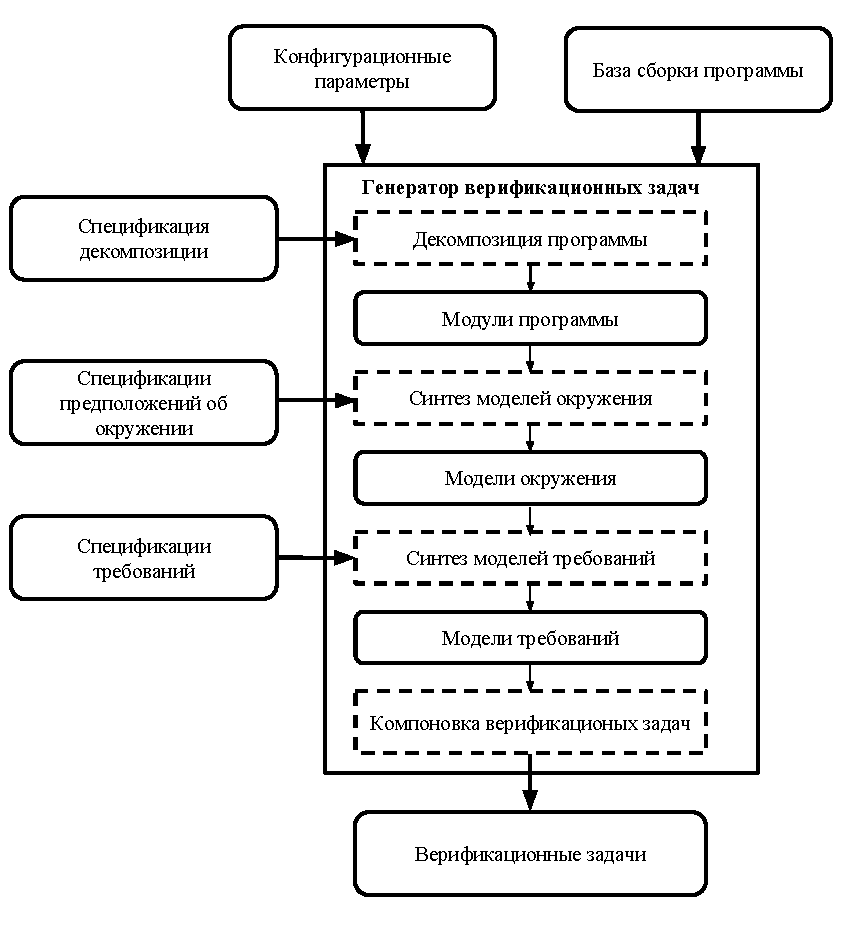
\includegraphics[scale=1]{vt_generator}
\caption{Схема генератора верификационных задач.}
\label{figure:vt_generator}
\end{figure}

Программные системы на языке Си, как правило, распространяются в виде файлов с исходным кодом и скриптов для их компиляции и компоновки.
Для получения информации об устройстве такой системы выполняется контролируемая сборка, в ходе которой подготавливается \textit{база сборки}.
В рамках данного метода процесс сбора такой базы не рассматривается и предлагается использовать для этого доступные инструменты.
База сборки должна содержать следующие данные в своем составе:
\begin{itemize}
    \item файлы с исходным кодом программной системы на языке программирования Си;
    \item команды компиляции и компоновки в виде графа зависимостей между командами сборки;
    \item описание программного интерфейса файлов программной системы.
    \end{itemize}
    
В базе сборки сохраняются все файлы программной системы с расширением <<.c>> и заголовочные файлы зависимостей, необходимые для выполнения препроцессирования.

Пример фрагмента графа зависимостей между командами сборки изображен на рисунке \ref{figure:cbg}.
Граф является ориентированным и его вершинам соответствуют файлы, которые являются входными и выходными файлами команд сборки, а ребра графа соответствуют самим командам сборки.
Граф должен включать не только команды компиляции и компоновки, но и команды перемещения, удаления, переименования файлов и т.п.
Наличие ребра в графе между двумя вершинами означает, что некоторая команда сборки принимает на вход исходный файл и получает на выходе новый файл.
В составе графа хранится вспомогательная информация о командах сборки, например, опции команд, путь к директории выполнения, значения переменных окружения.
Если граф построен корректно, то в графе нет ребер направленных к вершинам, которые соответствуют файлам с исходным кодом, а вершины, соответствующие финальным исполняемым файлам программной системы, не содержат исходящих ребер.

\begin{figure}
\centering
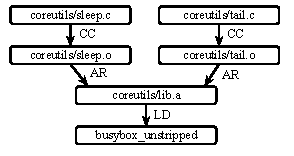
\includegraphics[scale=2]{cbg}
\caption{Фрагмент графа зависимостей команд сборки апплетов проекта BusyBox.}
\label{figure:cbg}
\end{figure}

Описание программного интерфейса программной системы представляет собой структурированные данные о составе каждого файла с исходным кодом, которые содержат:
\begin{itemize}
    \item Список деклараций и определений функций вместе с их сигнатурами.
    \item Граф вызова функций. Для каждого вызова должна быть сохранена информация о вызываемой и вызывающей функциях.
    Параметры вызова сохраняются в том случае, если среди них есть указатели на глобальные переменные или функции.
    \item Список инициализируемых глобальных переменных и их декларации.
    \item Список макросов и макроподстановок сохраняется аналогично списку определений и деклараций функций.
    \item Список определений и области видимости типов, определенных в программной системе.
\end{itemize}

Результатом работы генератора верификационных задач является набор верификационных задач в формате сообщества SV"~COMP.
Процесс генерации верификационных задач состоит из 4 шагов:
\begin{enumerate}
    \item На первом шаге в процессе декомпозиции определяются модули программной системы. 
    \item Затем для каждого модуля выполняется подготовка модели окружения на языке программирования Си.
    \item После моделей окружения синтезируются модели требований на языке программирования Си.
    \item Заключительным шагом является компоновка полученных на предыдущих шагах данных для получения верификационных задач в заданном формате.
\end{enumerate}

Каждый из перечисленных шагов выполняется отдельным компонентом генератора верификационных задач.
В рамках компонентов могут быть реализованы разные подходы и алгоритмы для выполнения конфигурирования в зависимости от проверяемых требований и программной системы.
Настройка процесса генерации верификационных задач выполняется согласно конфигурационным параметрам, заданным пользователем.

\section{Метод декомпозиции Си-программ на модули}
В данном разделе представлен метод автоматизированной декомпозиции Си-программ на модули, нацеленный на решение следующих задач:
\begin{itemize}
    \item выделить часть исходного кода программной системы, которую требуется верифицировать;
    \item декомпозировать выделенную часть исходного кода программной системы на модули, которые инструменты верификации моделей программ способны проверить по отдельности в составе верификационных задач.
\end{itemize}

Результат декомпозиции программной системы характеризуется следующими показателями:
\begin{itemize}
    \item \textit{Число полученных модулей}. Чем модулей меньше, тем, как правило, меньше времени потребуется на верификацию и ниже трудозатраты на моделирование окружения.
    \item \textit{Трудозатраты на моделирование окружения}. Трудозатраты зависят от сложности программного интерфейса модулей. Чем больше число точек входа и неопределенных функций в каждом модуле, тем больше моделей сценариев взаимодействия и неопределенных функций требуется подготовить пользователю.
    \item \textit{Число таких модулей, верификационные задачи на основе которых могут быть решены инструментом верификации моделей программ}.
\end{itemize}

Число точек входа и размер модулей лишь косвенно влияют на трудоемкость моделирования окружения и возможность решить верификационные задачи, построенные на основе модулей, в заданных ограничениях на вычислительные ресурсы при использовании определенного инструмента верификации моделей программ.
Трудоемкость моделирования окружения может оценить только пользователь, выполняющий верификацию, а вердикт станет известен только после непосредственного запуска инструмента верификации моделей программ.
Поэтому в данной работе предлагается выполнять процесс декомпозиции автоматически, но с возможностью конфигурирования и коррекции состава полученных модулей программы пользователем при помощи спецификации декомпозиции в зависимости от проверяемых требований и программы.

Для декомпозиции программной системы на языке Си предлагается выполнять следующие шаги:
\begin{enumerate}
    \item определить файлы и функции в составе программы;
    \item выделить модули;
    \item выбрать целевые модули;
    \item скорректировать состав модулей согласно спецификации декомпозиции;
    \item агрегировать модули.
\end{enumerate}

На шаге определения состава программы выполняется построение двух ориентированных графов на основе базы сборки: графа файлов и графа функций. 
Вершины графа функций соответствуют уникальным функциям, а ребро между вершинами присутствует в графе, если одна функция вызывается из другой.
Граф может не содержать тех функций, в которых нет вызова функций из других файлов программы и которые сами не вызываются за пределами файла с их определением.
Граф файлов строится таким образом, чтобы вершины соответствовали уникальным файлам с исходным кодом программы, а ребра связывали вершины, если хотя бы одна функция из файла вызывает некоторую функцию из другого файла.

На следующем шаге выполняется деление множества вершин графа файлов на непересекающиеся подмножества, согласно некоторой \textit{стратегии выделения модулей}.
При решении поставленной задачи могут использоваться данные из базы сборки, графа функций и графа файлов.
В результате декомпозиции должен быть получен граф модулей.
Вершиной графа является модуль программы --- это набор из одного или нескольких файлов программы.
Каждый файл программы должен быть частью некоторого модуля.
Между вершинами графа есть ребро, если есть хотя бы одно ребро в графе файлов между вершинами, которые соответствуют файлам из разных модулей.
Каждому модулю назначается уникальное имя.
Требуется, чтобы при верификации одной и той же версии программы с одними и теми же конфигурационными параметрами алгоритм получал всегда один и тот же граф модулей с одними и теми же именами вершин и составом каждого модуля.

Для каждой новой верифицируемой программы предлагается разрабатывать подходящую стратегию выделения логических компонентов.
Архитектура компонента декомпозиции программ должна позволять выделять общие между реализациями стратегий алгоритмы и функции, чтобы сократить трудоемкость разработки.

Шаг выделения модулей является необязательным и может быть пропущен на начальной стадии выполнения верификации или при проверке программ небольшого размера, для которых состав модулей нетрудно задать вручную при помощи спецификации декомпозиции.

Задачу декомпозиции графа файлов можно свести к строго математической задаче разбиения множества вершин графа на подмножества и использовать для ее решения различные существующие алгоритмы, не опирающиеся на особенности устройства декомпозируемых программных систем.
Данный подход может быть реализован в качестве одной из стратегий выделения модулей в рамках данного метода.
Трудность такого подхода заключается в определении способа формализации данной задачи таким образом, чтобы ее решение действительно способствовало улучшению показателей применимости метода на практике, то есть снижению показателя трудоемкости моделирования окружения и повышению числа верификационных задач, подготовленных на основе модулей, для которых возможно получить вердикт при заданных ограничениях на вычислительные ресурсы. 
Так как набора таких характеристик модуля, которые явно влияют на целевые показатели, предложить не удается, то и разные алгоритмы решения данной задачи оказываются применимы только в некоторых частных случаях.

Следующим шагом является выбор целевых модулей.
Пользователь в числе конфигурационных параметров может перечислить два списка имен директорий, файлов, функций или модулей.
Списки могут содержать и регулярные выражения для определения таких имен.
Один список перечисляет те объекты, которые требуется верифицировать, а другой те, которые верифицировать не требуется.
На шаге выбора целевых модулей должны быть помечены вершины графа модулей, которые требуется верифицировать на основе данных списков.
Для каждого заданного пользователем элемента списка определяется соответствующее множество целевых файлов: для директории все файлы с исходным кодом, включая и файлы из поддиректорий, для модулей все файлы из их состава, а для функции файл с ее определением.
Затем формируется множество целевых файлов, предназначенных для верификации, а затем из него вычитается множество элементов, полученных для списка имен объектов, которые следует исключить.
В результате должно быть сформировано непустое множество целевых файлов, которые требуется верифицировать, и каждая вершина графа файлов, соответствующая элементу данного множества, помечается как целевая.
Каждая вершина графа модулей тоже помечается как целевая, если соответствующий модуль содержит хотя бы один целевой файл.

Затем выполняется шаг коррекции состава модулей, который является необязательным и выполняется в том случае, если пользователь подготовил спецификацию декомпозиции.
Спецификация декомпозиции может содержать следующие команды:
\begin{itemize}
    \item Добавить или заменить состав файлов модуля с определенным именем.
    \item Добавить или удалить определенные файлы из модуля с некоторым именем.
    \item Удалить определенные файлы из всех модулей.
    \item Добавить определенные файлы ко всем модулям.
\end{itemize}

Для удобства пользователя следует предоставить возможность задавать не только имена файлов, но и функций, логических компонентов и директорий, а также поддержать использование регулярных выражений при задании спецификации декомпозиции.

На основе заданной пользователем спецификации декомпозиции выполняется коррекция вершин графа модулей, а затем на основе графа файлов заново определяются множества ребер графа модулей и его целевые вершины. 

Последним шагом является агрегация модулей.
На данном шаге выполняется для каждого целевого модуля поиск наборов модулей, которые могут включать и нецелевые модули, согласно некоторой \textit{стратегии агрегации}.
Стратегия реализует алгоритм для выбора модулей, чтобы либо снизить число точек входа целевого модуля, либо снизить число неопределенных функций при объединении модулей из набора в новый модуль.
Агрегация нацелена на сокращение трудоемкости моделирования окружения при помощи верификации модулей вместе.
При разработке стратегии стоит учесть, что увеличение числа наборов объединенных модулей приводит к увеличению времени верификации, а увеличение размера наборов повышает риск возникновения взрыва числа состояний в модели, построенной инструментом верификации на основе исходного кода объединенных модулей.

В рамках предложенного метода предлагается разработать несколько стратегий агрегации на основе различных алгоритмов.
Стратегии могут опираться не только на графы модулей, файлов и функций, но и на некоторую вспомогательную информацию, которую может предоставить пользователь.
Например, такими данными могут быть отчеты о покрытии, полученные при верификации модулей по-отдельности.

Каждый набор модулей, полученный в ходе агрегации, становится новым модулем, для которого затем выполняется синтез моделей окружения и требования.

\begin{figure}
\centering
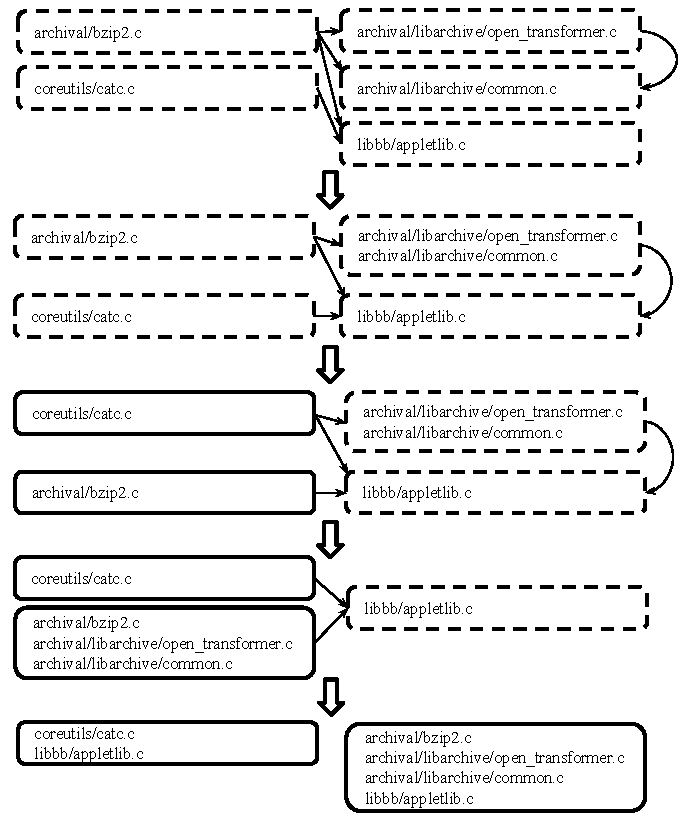
\includegraphics[scale=1.2]{decomposition_example}
\caption{Пример декомпозиции фрагмента проекта BusyBox на модули.}
\label{figure:decomposition_example}
\end{figure}

Рассмотрим процесс декомпозиции на примере, представленном на рисунке~\ref{figure:decomposition_example} и основанном на небольшой части проекта BusyBox.
Пример иллюстрирует результат работы каждого шага метода.
Прямоугольниками со сплошными границами представлены целевые модули, а нецелевые модули имеют пунктирные границы.
Стрелки соответствуют зависимостям по вызову функций между файлами и модулями.
\begin{itemize}
    \item Пусть после выполнения определения состава программы оказалось, что в программе 5 файлов, зависимости по вызову функций между которыми представлены на рисунке. 
    В данном примере файлы в левой части соответствуют апплетам \textit{bzip2} и \textit{catc}, каждый из которых имеет свою функцию \textit{main}.
    Файл из директории \textit{libbb} соответствует одноименной библиотеке функций, которая может быть использована любым апплетом.
    Файлы из директории \textit{archival/libarchive} реализуют вспомогательные функции для различных апплетов, предназначенных для сжатия и распаковки архивов.
    \item На втором шаге выполняется выделение модулей на основе некоторой стратегии.
    Пусть в данном примере стратегия на основе графа вызова функций предполагает объединение файлов из одной директории, отделяя друг от друга те модули, в которых в каждом есть своя функция \textit{main}.
    \item На третьем шаге выбираются целевые модули.
    В данном случае целевыми являются модули с файлами \textit{bzip2} и \textit{catc}, которые содержат функции \textit{main}.
    \item На предпоследнем шаге выполняется коррекция состава модулей согласно спецификации декомпозиции.
    Предположим, что пользователь указал, что для всех апплетов из \textit{archival} необходимо добавить файлы из\break \textit{archival/libarchive}, которые в свою очередь не нужно выделять в отдельный модуль.
    \item На заключительном этапе на основе графа вызова функций между модулями для сокращения затрат на моделирование окружения выполняется агрегация апплетов со вспомогательной библиотекой \textit{libbb}.
\end{itemize}

Предложенный метод позволяет адаптировать процесс декомпозиции для проверки различных программных систем на языке программирования Си.
Для этого предлагается разрабатывать стратегии выделения модулей и агрегации, а также спецификации декомпозиции.

\section{Метод спецификации моделей окружения}
В данном разделе представлен метод спецификации моделей окружения модулей на основе систем переходов.

\subsection{Промежуточная модель окружения}
После декомпозиции программы требуется для каждого модуля Си-программы подготовить модель окружения, которая состоит из моделей неопределенных функций и моделей сценариев взаимодействия.

Для преобразующих программ с функцией \textit{main} не требуется описывать разные последовательности вызова точек входа и прежде всего нужно разработать модели определенных в окружении функций на языке программирования Си.
В данной работе внимание сосредоточено именно на задаче моделирования сценариев взаимодействия, в которых выполняется вызов точек входа модулей.

Процесс моделирования окружения для библиотек и событийно-ориентированных программ требует построения композиции из отдельных моделей сценариев взаимодействия.
Объединение модулей программы при использовании стратегий агрегации ведет, как правило, к уменьшению трудозатрат на моделирование.
Однако при этом могут возникать новые ограничения на последовательности событий из разных сценариев взаимодействия.
Способ описания таких требований не должен препятствовать раздельной верификации модулей с одними и теми же моделями сценариев, то есть реализации таких моделей не должны существенным образом зависеть друг от друга.
Для решения данной задачи в настоящей работе предлагается метод задания моделей сценариев на основе систем переходов.
Спецификацию предположений об окружении для некоторого модуля программы, подготовленную при помощи данного метода, назовем промежуточной моделью окружения.

Способ описания промежуточной модели окружения должен удовлетворять ряду требований для удобства применения на практике:
\begin{itemize}
    \item Модели сценариев взаимодействия должны быть описаны отдельно друг от друга.
    \item Модели событий следует описывать на языке программирования Си. 
    Такой подход призван облегчить восприятие моделей пользователем и упростить их трансляцию на язык Си при подготовке финальной модели окружения.
    \item При агрегации нескольких модулей модель окружения в промежуточном представлении для группы модулей должна быть построена как параллельная композиция моделей сценариев, подготовленных для отдельных модулей.
    Каждая модель сценария описывает события взаимодействия, которые происходят в отдельном потоке окружения согласно семантике выполнения многопоточной программы в соответствии со стандартом POSIX.
\end{itemize}

Рассмотрим способ задания промежуточной модели окружения, не опираясь на конкретный синтаксис, который может быть реализован по-разному.
Пусть требуется разработать модель окружения для модуля программы на языке программирования Си с программным интерфейсом $I = <V_p, F_p, R_e, T_e>$, который содержит множества глобальных переменных, функций, макросов и типов, для которых известны сигнатуры, область видимости в файлах программы и файл с объявлением или определением.
Описание программного интерфейса может быть получено из базы сборки программы.

Промежуточную модель окружения данного модуля обозначим как $M$, где:
\[ M = <V_e, F_e, R_e, T_e, E> \]
Здесь $V_e, F_e, R_e, T_e$ --- это множества вспомогательных вспомогательных переменных, функций, макросов и типов.
Для переменных заданы объявления и инициализаторы, а для остальных элементов даны определения на языке программирования Си.
Пересечения перечисленных множеств с соответствующими множествами из $I$ могут быть непустыми.
$E$ содержит конечное множество моделей сценариев взаимодействия модуля программы и окружения.

Множество $F_e$ содержит определения моделей функций из окружения и \textit{служебных функций}.
Множества $R_e, T_e$ и $V_e$ являются вспомогательными и необходимы для реализации моделей функций окружения и моделей сценариев взаимодействия.
Служебные функции выполняют следующие задачи:
\begin{itemize}
    \item При помощи данных функций может быть выделена общая функциональность ряда моделей.
    \item Служебные функции могут реализовывать модели функций стандартной и других библиотек, которые необходимы при использовании определенных инструментов верификации моделей программ.
    К таким функциям относятся функции выделения памяти, работы со строками, механизмами синхронизации и др.
    \item Некоторые служебные функции служат для <<связывания>> моделей окружения и моделей требований. Подробнее этот вопрос рассматривается в разделе, посвященном синтезу моделей требований.
\end{itemize}

Множество моделей сценариев взаимодействия $E$ содержит модели сценариев, которые делятся на два вида: модели функций окружения и модели потоков окружения. 
Каждая модель функции окружения реализует модель сценария взаимодействия, события которого происходят во время выполнения некоторой функции окружения из $F_p \setminus F_e$. 
Модель потока окружения реализует модель сценария, события которого выполняются
в некотором отдельном потоке окружения.
Все модели потоков окружения в точке входа модели окружения начинают выполнение одновременно.

Каждая модель сценария определяется четверкой:
\[ \varepsilon = <\mathcal{V}, \mathcal{A}, \alpha_0 ,\mathcal{R}>\]
Где $\mathcal{V}$ --- это множество переменных состояния, а $\mathcal{A}$ --- это множество \textit{действий} $\mathcal{R}:~ \mathcal{A}~\times~\mathcal{A}$ --- отношение переходов, описывающее допустимый порядок следования действий.

Модель сценария всегда начинается с выполнения действия $\alpha_0$, а последующие действия определяются отношением переходов $\mathcal{R}$. 
Будем различать действия трех видов: \textit{прием} и \textit{отправка} сигналов, а также \textit{модели событий}.

Модели событий предназначены для вызова точек входа и выполнения операций с их параметрами.
Модель события определяется тройкой:
\[\alpha = <\varphi, \beta, \psi> \]
Где $\beta$ --- это базовый блок кода на языке программирования Си, состоящий из операций над переменными $\mathcal{V} \cup V_p \cup V_e$, в котором могут быть вызваны функции из $F_p$ и $F_e$.
Базовый блок должен содержать корректный код и иметь один вход и один выход, то есть, если в блоке есть операторы ветвления или циклов, то они полностью должны входить в состав блока.
В базовых блоках запрещено объявлять новые переменные и использовать оператор $goto$.
Логические выражения $\varphi$ и $\psi$ на языке программирования Си над переменными $\mathcal{V}_i \cup V_p \cup V_e$ описывают предусловия и постусловия действия.

Действия передачи сигналов служат для описания зависимостей по порядку и данным между моделями событий из разных сценариев.
Рассмотрим модель сценария $\varepsilon_i$ с действием отправки сигнала и модель сценария $\varepsilon_j$ с действием получения сигнала.
Соответствующие действия $\alpha_i \in \mathcal{A}_i$ и $\alpha_j \in \mathcal{A}_j$ имеют вид:
\begin{align*}
&\alpha_i = <\varphi_i, \varepsilon_i, l_m>
&\alpha_j = <\varphi_j, \pi_j, l_n, \psi_j>    
\end{align*}
Константы $l_m$ и $l_n$ называются именами сигналов.
Передача сигнала возможна только тогда, когда в соответствующих действиях отправки и получения указано одно и то же имя сигнала $l_m = l_n$.
Логические выражения $\varphi_j$ и $\psi_j$ на языке программирования Си над переменными из $\mathcal{V}_j \cup V_p \cup V_e$ определяют предусловие и постусловие приема сигнала.
Предусловие посылки сигнала является логическим выражением $\varphi_i$, определенным на множестве переменных $\mathcal{V}_i \cup V_p \cup V_e$.
Два набора переменных $\varepsilon_i: {v_1, ..., v_k}$ где $t = 1..k, v_t \in \mathcal{V}_i$ и $\pi_j: {u_1, ..., u_k}$ где $t = 1..k, u_t \in \mathcal{V}_j$ предназначены для передачи значений между переменными состояния отправителя и получателя:
\begin{align*}
&\forall t = 0..k:~v_t := u_t
\end{align*}
Типы переменных должны либо совпадать, либо допускать преобразование.

Посылка сигнала происходит между одним получателем и одним отправителем согласно модели синхронизации потоков рандеву, предложенной в работе~\cite{Hoare:1978:CSP}.
Передача происходит между двумя моделями сценариев, одна из которых отправляет сигнал, а другая получает, причем имя сигнала в заданных действиях должно совпадать.
Для этого получатель должен выполнить действие получения сигнала, разрешенное отношением переходов, а отправитель выполнить соответствующее действие посылки сигнала.
Как только и отправитель, и получатель начали выполнять соответствующие действия, то может быть произведена передача данных.
После передачи данных отправитель может продолжать выполнение других действий, а получатель продолжит свою работу только после получения данных, которое может произойти не одновременно с отправкой.
Отправитель или получатель могут предпринять и другие действия, допустимые отношением переходов, независимо от наличия потенциальных получателей или отправителей.
Если же отношение переходов не разрешает выполнение других действий кроме посылки или отправки сигнала, то никаких действий в модели сценария выполняться не должно до появления необходимой пары для передачи сигнала.
Если потенциальных получателей или отправителей несколько, то пересылка сигнала происходит согласно недетерминированному выбору двух участников, а остальные модели сценариев, которые должны выполнить посылку или отправку сигнала с тем же именем, ожидают завершения передачи сигнала.

Модели сценариев можно описывать на языке программирования Си, как и остальные части промежуточной модели окружения $M$.
В этом случае каждая модель сценария может быть определена при помощи функции, в которой будут объявлены переменные состояния, а порядок действий может быть задан при помощи операторов языка.
Для действий посылки и получения сигналов предлагается расширить язык Си вспомогательными операциями для удобства спецификации.
Но и данные операции можно транслировать на язык Си, что будет описано в следующем разделе.
При реализации метода синтеза моделей окружения для задания моделей сценариев промежуточной модели окружения могут быть использованы и дополнительные расширения языка Си для решения ряда задач, возникающих на практике для преодоления ограничений инструментов верификации моделей Си-программ.

При спецификации промежуточной модели окружения целесообразно использовать специальные поддерживаемые инструментами верификации функции.
Поэтому исходный код модели окружения не предназначен для выполнения и служит только для компоновки с исходным кодом модуля программы в рамках верификационной задачи.

Семантика выполнения модели окружения без исходного кода модуля не имеет смысла, так как модель окружения предназначена для того, чтобы дополнить исходный код модуля до структурно-полной программы на языке Си.
В такой программе только одна точка входа и неопределенными могут быть только некоторые функции стандартной библиотеки и те функции, для которых инструмент верификации имеет встроенную модель.

\subsection{Пример промежуточной модели окружения}
Рассмотрим пример промежуточной модели окружения для модуля подсистемы.
Для задания моделей сценариев промежуточной модели окружения будем использовать язык Си, в котором будут добавлены расширения для обозначения действий передачи и получения сигналов.
Операции для посылки и приема сигнала $A$ пусть имеют вид $send(A, p1, ..., pN);$ и \break $receive(A, p1, ..., pN);$ соответственно.
Порядок действий будем задавать при помощи условного оператора и функции \textit{\_\_VERIFIER\_nondet\_int}, а предусловия и постусловия будут заданы при помощи функции \textit{\_\_VERIFIER\_assume}.
Такой способ несколько затрудняет восприятие, зато позволяет строго обозначить начало и конец описания каждого действия, которые будем сопровождать соответствующими комментариями.

Для данного модуля был предложен пример модели окружения, которая состояла из моделей сценария вызова библиотечных функций и сценария инициализации подсистемы.
Модель сценария инициализации подсистемы пусть имеет вид:

\begin{lstlisting}[language=C,basicstyle=\small]
void init_scenario(void) {
    // State vars
    int ret;

    // Transition Relation    
    // Block Action 1 begin
    ret = tty_init();
    // Block Action 2 end
    if (__VERIFIER_nondet_int()) {
        // Send Action 2 begin
        __VERIFIER_assume(ret == 0);
        send("INITIALIZED");
        // Send Action 2 end
    }
}
\end{lstlisting}

Здесь при помощи комментариев на языке Си обозначены конкретные части описания сценария: переменные состояния, операторы отношения переходов и действия.
Первое действие является блоком кода, в котором выполняется вызов функции инициализации подсистемы.
А второе действие с предусловием, выраженным при помощи вызова функции \textit{\_\_VERIFIER\_assume}, отправляет сигнал для активации сценария вызова библиотечных функций, который в свою очередь может быть задан следующим образом:

\begin{lstlisting}[language=C,basicstyle=\small]
void functions_scenario(void) {
    // State vars
    int ret;
    struct tty_driver *driver;
    struct tty_operations *ops;
    
    // Transition Relation
    // Receive Action 1 begin
    receive("INITIALIZED");
    // Receive Action 1 end
    // Block action 2 begin
    driver = tty_alloc_driver(...)
    // Block action 2 end
    if (__VERIFIER_nondet_int()) {
        // Block action 3 begin
        __VERIFIER_assume(driver != 0);
        ops = __VERIFIER_nondet_pointer();
        tty_set_operations(driver, ops);
        // Block action 3 end
        // Block action 4 begin
        ret = tty_register_driver(driver)
        // Block action 4 end
        if (__VERIFIER_nondet_int()) {
            // Send Action 5 begin
            __VERIFIER_assume(ret == 0);
            send("Register TTY callbacks", driver);
            // Send Action 5 end
            // Receive Action 6 begin
            receive("Unregister TTY callbacks", driver);
            __VERIFIER_assume(driver->ops == ops);
            // Receive Action 6 end
            // Block action 7 begin
            tty_unregister_driver(driver);    
            put_tty_driver(driver);
            // Block action 7 end
        } else {
            // Block action 8 begin
            __VERIFIER_assume(ret != 0);
            // Block action 8 end
        }
    }    
}
\end{lstlisting}

Первым действием сценария является прием сигнала, который означает, что подсистема инициализирована.
Затем выполняется вызов точек функций подсистемы.
Отличительной особенностью данной модели по сравнению с моделью окружения на языке Си, которая была предложена в первом разделе данной главы, является посылка и ожидание сигналов \textit{Register TTY callbacks} и \textit{Unregister TTY callbacks} после успешного вызова функции \textit{tty\_register\_driver}.
Данные действия указаны для демонстрации того, как указание о возможности вызова обработчиков драйверов может быть передано соответствующим моделям сценариев.
Данная модель сценария ожидает сигнал \textit{Unregister TTY callbacks}, который означает, что вызов обработчиков драйверов завершен.
Если в промежуточной модели окружения нет моделей сценариев, которые отправляют или принимают сигналы \textit{Register TTY callbacks} и \textit{Unregister TTY callbacks}, то они могут быть удалены из рассматриваемой модели вызова библиотечных функций при трансляции на язык Си.

\subsection{Трансляция промежуточных моделей окружения}
Модели сценариев, согласно предложенному методу, можно описывать на языке программирования Си, но для описания действий посылки и получения сигналов предлагается расширить язык Си вспомогательными операциями для удобства спецификации.
Поэтому промежуточные модели окружения должны быть предварительно транслированы на язык программирования Си. 
Тогда нужно показать, что трансляция промежуточной модели окружения не влияет на возможность обнаружения ошибок в модуле.

Модель окружения на языке программирования Си анализируется в рамках верификационной задачи инструментом верификации моделей программ при проверке некоторого свойства корректности.
Под программой далее будем понимать именно совокупность исходного кода модели окружения и модуля программы.
По исходному Си-программы строится модель, которая проверяется на соответствие свойству недостижимости ошибочных состояний\footnote{В данной работе рассматриваются только такие свойства корректности, которые могут быть сведены к задаче недостижимости ошибочного оператора.} методом верификации моделей.
Покажем, что множества ошибочных состояний исходной программы и программы, полученной после трансляции исходной программы на язык Си, изоморфны.
Для этого необходимо рассмотреть свойства таких моделей рассматриваемых программ, которые используются инструментами верификации моделей при проверке свойств недостижимости ошибочного оператора.

\subsubsection{Символическая система переходов}

Для описания моделей программ воспользуемся символическими системами переходов (англ. symbolic transition system)~\cite{Clarke:1981}.
Система определяется тройкой $STS \mathbf{:=} <V, \alpha, \delta>$. Где $V$ --- конечное множество типизированных переменных системы, каждая из которых задана на дискретном конечном множестве значений.
Функция означивания $s \in \Sigma_V$ переменных из множества $V$ называется состоянием системы. Множество $\Sigma_V$ --- это множество состояний системы, полученное перебором всех возможных значений переменных из множества $V$.
Формула пропозициональной логики $\alpha(V)$ над переменными из множества $V$ называется \textit{характеристической функцией множества начальных состояний}.
Состояния, при которых данный предикат принимает истинное значение, называются \textit{начальными состояниями}.
Формула пропозициональной логики $\delta(V, V^{'})$ --- это \textit{характеристическая функция отношения переходов} между состояниями.
Функция определена над переменными из $V \cup V^{'}$, то есть переменными в данном и в следующем состояниях системы.
Если для двух состояний $s_1 \in \Sigma_V$ и $s_2 \in \Sigma_V$ выполняется $(s_1, s_2) \models \delta$, то между ними возможен переход.

\textit{Путь} --- это конечная последовательность $\xi_k = s^0, s^1, ..., s^k$ состояний \break $s^{i} \in \Sigma_{V}$, в которой для каждого состояния справедливо $(s^{i}, s^{i+1}) \models \delta$ и для начального состояния $s^1 \models \alpha$. 
\textit{Предикат пути} длины $k$ шагов имеет вид:

\[
\eta_k \mathbf{:=} \alpha(V^{1}) \land \bigwedge_{i \in [1,k]}\delta[V = V^{i}, V^{'} = V^{i+1}](V, V^{'})
\]

$V^{i}$ обозначает множество переменных системы на шаге выполнения $i$.
Будем говорить, что состояние $s^k \in \Sigma_{V}$ достижимо за $k$ шагов, если существует такой путь выполнения $\xi_k = {s^1, s^2, ... s^k}$, что $\xi_k \models \eta_k$.
Обозначим множество всех достижимых за $k$ шагов состояний как $R_k$, а множество всех достижимых состояний как $R$.

Рассмотрим некоторое подмножество переменных системы $U \subseteq V$.
Проекцией состояния $s \in \Sigma_{V}$ на множество переменных $U$ называется такая функция означивания переменных $U$, обозначаемая как $s \Downarrow U$, которая переменным из $U$ ставит в соответствие те же значения, что и $s$.
Проекцией $K \Downarrow U$ некоторого подмножества всех состояний системы $K \subseteq \Sigma_V$ на множество переменных $U$ назовем множество всех проекций состояний из $K$ на множество переменных $U$.


\subsubsection{Символическая система переходов и структуры Крипке}
Каждый способ моделирования систем <<фиксирует>> свой набор свойств системы.
Метод описания систем при помощи структур Крипке широко распространен и применяется в том числе и для проверки свойства недостижимости ошибочных состояний.
Метод моделирования систем при помощи систем символических переходов не уступает в выразительности структурам Крипке.

Построим следующую структуру Крипке про произвольной $STS$:
\[K \mathbf{:=} <S, S_0, R, L>\]

\begin{itemize}
    \item $S = \Sigma_V$ --- конечное множество абстрактных состояний, полученное путем рассмотрения всех значений переменных $V$.
    \item $S_0 = \{s \in S| s \models \alpha\}$ --- множество начальных состояний, удовлетворяющих характеристической функции $\alpha$.
    \item $R = \{(s, t)| (s, t) \models \delta\}$ --- отношение переходов, которое определяется определяется характеристической функцией $\delta$.
    \item $L(s)$ --- такая функция разметки, которая ставит в соответствие состоянию набор истинных предикатов из $AP = \{a_1, ..., a_k\}$, определенных на множестве переменных $V$. То есть $a_i \in L(s)$, если $s \models a_i$.
\end{itemize}

В построенной структуре Крипке $K$ и в $STS$ множества всех состояний системы, начальных состояний и переходов попарно совпадают.
То есть для любой символической системы переходов может быть построена эквивалентная структура Крипке.

\subsubsection{Язык программирования $LZ$}

Расширения языка Си для отправки и получения сигналов влияют на порядок выполнения операций в программе и передачу данных между потоками.
Предположим, что и при трансляции новых операций на язык Си будут использоваться некоторые только операции с целыми числами, захват и освобождение блокировок, проверка простых логических выражений.
При посылке и получении сигналов, а также при трансляции данных операций на язык Си, не предполагается использовать вызовы произвольных функций, циклы с переменным числом итераций, рекурсию, изменять значения по указателям, выделять или освобождать память, создавать или останавливать потоки, выполнять переходы по goto и т.п.
Поэтому при рассмотрении программ и их моделей целесообразно рассмотреть упрощенный Си-подобный язык, который сохранит именно те особенности семантики программ на языке Си, на которые влияет добавление операций посылки и получения сигналов.
Таким языком станет некоторый структурный статически типизированный язык программирования $LZ$.

Программа на языке $LZ$ имеет следующий синтаксис:
\begin{flalign*}
& Globals:~g_1:~\tau_1;~g_2:~\tau_2;~...~g_n:~\tau_n;\\
& Procedures: \\
& ~~~Procedure~1:\\
& ~~~~~~Locals:~v_1:~\tau_1;~v_2:~\tau_2;~...~v_{k_1}:~\tau_{k_1}; \\
& ~~~~~~P_1; \\
\\
& ~~~Procedure~2:\\
& ~~~~~~Locals:~v_2:~\tau_1;~v_2:~\tau_2;~...~v_{k_2}:~\tau_{k_2}; \\
& ~~~~~~P_2; \\
& ~~~... \\
& ~~~Procedure~N:\\
& ~~~~~~Locals:~v_2:~\tau_1;~v_2:~\tau_2;~...~v_{k_N}:~\tau_{k_N}; \\
& ~~~~~~P_N; \\
\end{flalign*}

Здесь использовались следующие обозначения:
\begin{itemize}
    \item $g_i$ --- глобальные переменные программы с типами $\tau_i$. Множества значений типов $\{int, lock, bool\}$ являются конечными и дискретными. Тип $int$ соответствует подмножеству целых чисел, $bool$ соответствует истинностным значениям, множество значений типа $lock$ содержит два элемента: 0 (блокировка не захвачена) и 1 (блокировка захвачена). \item $Procedure~i$ --- заголовок описания процедуры с номером $i$, которое состоит из деклараций локальных переменных $v_i$ и кода $P_i$ процедуры.
\end{itemize}

Выполнение программы представляет собой параллельное выполнение операций из процедур программы в отдельных потоках. 
Каждый $i$-ый поток выполняет соответствующую ему процедуру $P_i$.
Потоков в программе всегда не менее 1 и все они начинают выполнение одновременно.
Порядок выполнения операций одной процедуры определяется операторами следования ($;$), ветвления ($if$) и цикла ($while$).

Грамматика кода процедуры $P_i$ имеет вид:
\begin{flalign*}
P \mathbf{:=} &~P;P~|~if~(A)~\{P\}~else~\{P\}~|~while~(A)~\{P\}~|~op~|~skip \\
op \mathbf{:=} &~x = t~|~lock(x)~|~unlock(x)~|~assume(A) \\
t \mathbf{:=} &~(t)~|~t - t~|~x~|~t + t \\
A \mathbf{:=} &~\neg A~|~A \land A~|~A \lor A~|~A \to A~|~(A)~|~x~|~nondet()
\end{flalign*}

Рассмотрим каждый символ подробнее:
\begin{itemize}
    \item $op$ --- операция в программе. Операциями являются $lock$, $unlock$, $assume$, $skip$ и присваивание.
    \item t --- выражение, составленное при помощи арифметических операторов \{+, -\} над переменными программы с типом $int$. Выражения используются только в операциях присваивания.
    \item x --- имя некоторой переменной. В любой процедуре может выполняться доступ к глобальным переменных и локальным переменным данной процедуры. Локальные переменные могут иметь только типы $int$ и $bool$.
    \item $lock(x)$ и $unlock(x)$ --- функции захвата и освобождения блокировки $x$. Блокировками являются глобальные переменные с типом $lock$.
    \item nondet() --- неопределенное значение из множества значений типа $bool$;
    \item $A$ --- логическая формула пропозициональной логики, расширенная теорией целых чисел. Формула может быть составлена при помощи логических связок $\{!, \&\&, ||, ==\}$ над переменными программы;
    \item $assume(A)$ --- проверка выполнения формулы $A$. Если формула не истинна, то процедура не может продолжить выполнение и перейти к следующей операции.
    \item $skip$ --- операция бездействия.
\end{itemize}

\subsubsection{Модель программ на языке программирования $LZ$}
Построим модель программы $P$ на языке $LZ$ при помощи символической системы переходов $STS \mathbf{:=} (V_P, \alpha_P, \delta_P)$.

В каждой процедуре пронумеруем каждую операцию и проверку условий циклов и операторов ветвления.
В результате каждая операция и условие операторов цикла или ветвления будут иметь свой уникальный порядковый номер, называемый \textit{меткой}.
Дополнительной меткой обозначим конец каждой процедуры.

Введем следующие обозначения:
\begin{itemize}
    \item $V_P = V \cup PC$--- множество переменных состояния.
    \item $\Sigma_{V_P}$ --- множество всех состояний модели программы.
    \item $V = G \cup L_0 \cup ... \cup L_N$ --- множество переменных.
    \item $G$ --- множество глобальных переменных программы.
    \item $L_i$ --- множество локальных переменных процедуры с номером $i$. 
    $V_i = G \cup L_i$ --- множество переменных процедуры $i$.
    \item Переменные $pc_i$ (англ. program counter) являются вспомогательными и предназначены для сохранения метки текущей выполняемой операции или проверяемого условия оператора. Множество таких переменных обозначим как $PC = \{pc_1, ... , pc_N\}$. 
    Элементы множества $C \subset \Sigma_{PC}$ всех допустимых функций означивания переменных $PC$ будем называть конфигурациями, а $\Sigma_{PC}$ множеством конфигураций.
    \item $\alpha_{P}(V_P)$ --- характеристическая функция начальных состояний.
    \item $\delta_{P}(V_{P}, V^{'}_{P})$ --- характеристическая функция отношения переходов.
\end{itemize}
 
Выполнение программы будем моделировать как асинхронную параллельную композицию потоков.
Характеристическая функция отношения переходов имеет вид:

\begin{flalign*}
& \delta_P(V_P, V^{'}_P) \mathbf{:=} \bigvee_{i \in [1,N]}(\delta_{i}(V_i, pc_i, V^{'}_i, pc_i^{'}) \land \sigma_i)\text{, где}  
\\
& \sigma_i \mathbf{:=} \bigwedge_{\substack{j \in [1,N],\\j \neq i}}same(\{pc_j\}\cup L_j)
\end{flalign*}

Здесь предикат $same(A)$ означает, что переменные из некоторого подмножества переменных состояния $A \subset V_P$ сохраняют свои значения:

\[same(A) \mathbf{=} \bigwedge_{x \in A}x^{'} = x\]

\textit{Характеристическая функция процедуры} $\delta_{i}(V_i, pc_i, V_i^{'}, pc_i^{'})$ моделирует выполнение отдельного потока с номером $i$.
Пусть поток выполняет процедуру $P_i$, в которой $k_i$ меток, тогда: 

\begin{align*}
\delta_{i}(V_i, pc_i, V^{'}_i, pc_i^{'}) \mathbf{:=} \bigvee_{l \in [1,k_i]}\delta_{op_l}(V_i, pc_i, V^{'}_i, pc_i^{'})
\end{align*}

Где $\delta_{op_l}$ --- \textit{характеристическая функция операции или оператора с меткой $l$}.
Пусть операция имеет метку $l_1$, а метка следующей выполняемой операции или условия оператора будет $l_2$.
Тогда характеристическая функция операции в позиции $l_1$ имеет вид:

\begin{align*}
\delta_{op_{l_1}}(V_i, pc_i, V'_i, pc'_i) \mathbf{:=} pc_i = l_1 \land pc'_i = l_2 \land \rho_{op}(V_i, V'_i)
\end{align*}

Здесь $\rho_{op}(V_i, V'_i)$ --- \textit{характеристическая функция операции}, которая не зависит от метки.
Характеристические функции операций языка представлены в таблице~\ref{table:predicate}.
 
Рассмотрим проверку условия $A(V_i)$ оператора ветвления или цикла с меткой $l_1$.
Если условие истинно, то выполнеются операция с меткой $l_{true}$, а иначе операция с меткой $l_{false}$.
Тогда характеристическая функция условия оператора с меткой $l_1$ имеет вид:

\begin{align*}
\delta_{op_{l_1}}(V_i, pc_i, V'_i, pc'_i) \mathbf{:=} & pc_i = l_1 \land same(V_i) \land \\
& (A(V_i) \land pc' = l_{true} \lor \neg A(V_i) \land pc' = l_{false})
\end{align*}

\begin{table}
\centering
\begin{tabular}{ | l | l |}
\hline
Операция & Характеристическая функция \\
\hline
$lock(x)$ & $\rho_{op}(V_i, V'_i) \mathbf{:=} x = 0 \land x' = 1 \land same(V_i \setminus \{x\}))$ \\
\hline
$unlock(x)$ & $\rho_{op}(V_i, V'_i) \mathbf{:=} x' = 0 \land same(V_i \setminus \{x\})$ \\
\hline
$x = t(V_i)$ & $\rho_{op}(V_i, V'_i) \mathbf{:=} x' = t(V_i) \land same(V_i \setminus \{x\})$ \\
\hline
$assume(A(V_i))$ & $\rho_{op}(V_i, V'_i) \mathbf{:=} A(V_i) \land same(V_i)$ \\
\hline
$skip$ & $\rho_{op}(V_i, V'_i) \mathbf{:=} same(V_i)$ \\
\hline
\end{tabular}
\caption{Характеристические функции операций языка $LZ$.}
\label{table:predicate}
\end{table}

Пусть в процедуре $i$ есть некоторый блок кода, состоящий из нескольких операций.
Первая операция блока всегда имеет \textit{метку входа в блок}, а \textit{метку выхода из блока} имеет следующий оператор после последнего оператора блока.
Здесь и далее блок кода всегда имеет только одну \textit{метку входа в блок} и одну \textit{метку выхода из блока}.
Пусть блок имеет метку входа $l_1$ и метку выхода из блока $l_2$.
\textit{Предикат пути через блок} имеет вид:

\begin{flalign*} 
\pi \mathbf{:=} pc^{1}_{i} = l_1 \land pc^{k+1}_{i} = l_2 \land \bigwedge_{i \in [1,k]}\delta_{P}[V_P = V^{i}_{P}, V^{'}_P = V^{i+1}_{P}](V_{P}, V^{'}_{P})
\end{flalign*}

Предикат $\Delta_k = \bigwedge_{i \in [1,k]}\delta_{P}[V_P = V^{i}_{P}, V^{'}_P = V^{i+1}_{P}](V_{P}, V^{'}_{P})$ будем называть \textit{предикатом шагов} и для краткости записывать как $\Delta_k = \bigwedge_{i \in [1,k]}\delta_{P}(V^{i}_{P}, V^{i+1}_{P})$.
Другую часть предиката пути назовем \textit{предикатом граничных условий} и обозначим $\gamma = pc^{1}_{i} = l_1 \land pc^{k+1}_{i} = l_2$.

Предикат моделирует путь длины $k$ шагов из состояния $s^1$, которое является функцией означивания переменных состояния $V^1_P$ на первом шаге, в состояние $s^{k+1}$, которое является функцией означивания переменных состояния $V^{k+1}_P$ после выполнения шага $k$.
Состояние $s^1$ будем называть \textit{входным}, а состояние $s^{k+1}$ \textit{выходным}.
Если существует такая конечная последовательность состояний $s^0, s^1, ..., s^k$, что предикат принимает истинное значение, то будем говорить, что состояние $s^{k+1}$ достижимо из состояния $s^{1}$ и обозначим этот факт как $(s^1, s^{k+1}) \models \pi$.

Рассмотрим блоки с предикатами пути $\pi_1$ и $\pi_2$ из разных программ с множествами состояний $\Sigma_{V_{P_1}}$ и $\Sigma_{V_{P_2}}$ соответственно.
Пусть программы имеют общее непустое множество переменных $U$, значения которых определяют ошибочные состояния.
Тогда блоки считаются эквивалентными относительно $U$, если для любых входного и достижимого выходного состояний $x_1$ и $y_1$ найдется путь через второй блок из состояния $x_2$ в $y_2$, у которых соответствующие проекции на множество переменных $U$ попарно совпадают с $x_1$ и $y_1$.
И выполняется условие, что второй блок не добавляет новых достижимых состояний с другими проекциями на множество $U$, которых в первом блоке быть не могло.

Условие эквивалентности блоков относительно множества переменных $U$ имеет вид:
\begin{enumerate}
    \item Для любого такого входного и выходного состояний $\{x_1$, $y_1\} \subset \Sigma_{V_{P_1}}$, что $(x_1, y_1) \models \pi_1$, найдутся такие входное и выходное состояния $\{x_2, y_2\} \subset \Sigma_{V_{P_2}}$ и $(x_2, y_2) \models \pi_2$, что $x_1 \Downarrow U = x_2 \Downarrow  U$ и $y_1 \Downarrow U = y_2 \Downarrow  U$.
    \item Для любого такого входного и выходного состояния $\{x_2, y_2\} \subset \Sigma_{V_{P_2}}$, что $(x_2, y_2) \models \pi_2$, найдутся входное и выходное состояния $\{x_1$, $y_1\} \subset \Sigma_{V_{P_1}}$ и $(x_1, y_1) \models \pi_1$, что $x_1 \Downarrow U = x_2 \Downarrow  U$ и $y_1 \Downarrow U = y_2 \Downarrow  U$.
\end{enumerate}

Рассмотрим случай последовательного выполнения двух некоторых операций с характеристическими функциями $\rho_1(x, x^{'})$ и $\rho_2(x, x^{'})$.
Операции имеют метки $1$ и $2$ соответственно, а после следует операция с меткой 3.
Путь через такой блок всегда имеет длину 2 шага и предикат пути имеет вид:
\begin{flalign*}
\pi\mathbf{:=} 
& pc^1 = 1 \land pc^3 = 3 ~\land \\
& (pc^1 = 1 \land \rho_1(V^1_i, V^2_i) \land pc^2 = 2 ~\lor \\ 
& ~pc^1 = 2 \land \rho_2(V^1_i, V^2_i) \land pc^2 = 3) ~\land \\
& (pc^2 = 1 \land \rho_1(V^2_i, V^3_i) \land pc^3 = 2) ~\lor \\ 
& ~pc^2 = 2 \land \rho_2(V^2_i, V^3_i) \land pc^3 = 3) \Leftrightarrow \\ 
& pc^1 = 1 \land pc^3 = 3 \land \rho_1(V^1_i, V^2_i) \land \rho_2(V^2_i, V^3_i) \end{flalign*}

Данный результат иллюстрирует возможность сокращенной записи предиката последовательного выполнения пути через блок.
Такой путь можно рассматривать как выполнение некоторой искусственной операции с характеристической функцией $\rho_{op}(V_i, V'_i) = \rho_1(V_i, V_t) \land \rho_2(V_t, V'_i)$, где $V_t$ --- вспомогательный набор переменных.
Такую функцию назовём \textit{предикатом блока}.
Предикат блока из $k$ последовательных операций имеет вид $V_i=V^{1}_i \land V^{'}_i = V^{k+1}_i \land \bigwedge{j \in [1,k]}\rho_i(V^j_i, V^{j+1}_i)$.

Рассмотрим оператор ветвления с условием $\phi(V_i)$ и ветвями, в которых выполняются блоки кода с предикатами $\rho_{then}$ и $\rho_{else}$ и метками $1$ и $2$. 
Метка выхода из блока пусть равна $4$.
Тогда предикат пути через блок с оператором ветвления имеет вид:
\begin{flalign*}
\pi \mathbf{:=} & pc^1 = 1 \land pc^3 = 4 ~\land \\
& (pc^1 = 1 \land ( \phi(V^1_i) \land pc^2 = 2 \lor \neg \phi(V^1_i) \land pc^2 = 3) \land V^2_i = V^1_i ~\lor \\ 
& ~pc^1 = 2 \land \rho_{then}(V^1_i, V^2_i) \land pc^2 = 4 \lor \\ &
~pc^1 = 3 \land \rho_{else}(V^1_i, V^2_i) \land pc^2 = 4) \land \\ &
(pc^2 = 1 \land (\phi(V^2_i) \land pc^3 = 2 \lor \neg \phi(V^2_i) \land pc^3 = 3) \land V^3_i = V^2_i \lor \\ &
~pc^2 = 2 \land \rho_{then}(V^2_i, V^3_i) \land pc^3 = 4 \lor \\ &
~pc^2 = 3 \land \rho_{else}(V^2_i, V^3_i) \land pc^3 = 4) \Leftrightarrow \\ &
pc^1 = 1 \land pc^3 = 4 \land V^2_i=V^1_i \land \\ &
(pc^2 = 2 \land \phi(V^1_i) \land \rho_{then}(V^1_i, V^3_i) \lor pc^2 = 3 \land \neg \phi(V^1_i) \land \rho_{else}(V^1_i, V^3_i))
\end{flalign*}

Предикат пути через блок с ветвлением можно рассматривать как выполнение за один шаг искусственной операции с характеристической функцией $\rho_{op}(V_i, V'_i) = \phi(V_i) \land \rho_{then}(V_i, V'_i) \lor \neg \phi(V_i) \land \rho_{else}(V_i, V'_i)$.
Такую функцию также будем называть предикатом блока.

Предикат последовательного пути через любой блок с операторами ветвления и следования можно представить в виде выполнения за один шаг искусственной операции с предикатом пути, построенным на основе правил, проиллюстрированных для отдельных двух операций и оператора ветвления.

Назовем операции \textit{независимыми}, если для их характеристических функций $\rho_1(V_i, V'_i)$ и $\rho_2(V_i, V'_i)$  справедливо условие: 

\begin{flalign*}
\rho_1(V^1_i, V^2_i) \land \rho_2(V^2_j, V^3_j) \Leftrightarrow \rho_2(V^1_j, V^2_j) \land \rho_1(V^2_i, V^3_i).
\end{flalign*}

Примером независимых операций являются операции над локальными переменными из разных потоков или операции, в результате которых изменяемая глобальная переменная имеет одно и то же значение.

\begin{lemma}
\label{interleaving}
Истинность предиката пути, на котором могут выполняться подряд две независимые операции не зависит от порядка выполнения данных операций между собой.
\end{lemma}
\begin{proof}
Утверждение тривиально выполняется для последовательного случая, если рассмотреть предикат блока из двух независимых операций:

\begin{flalign*}
\rho(V_i, V'_i) = & \rho_1(V_i, V_t) \land \rho_2(V_t, V'_i) \Leftrightarrow \rho_2(V_i, V_t) \land \rho_1(V_t, V'_i)
\end{flalign*}

Теперь рассмотрим два потока, в которых выполняются независимые операции c характеристическими функциями $\rho_1(V_1, V'_1)$ и $\rho_2(V_2, V'_2)$ соответственно.
Пусть обе операции имеют метку 1 в соответствующих процедурах, после которой следует метка 2.
Тогда предикат пути через блок имеет вид:

\begin{flalign*}
\pi \mathbf{:=} & pc^{1}_1 = 1 \land pc^{1}_2 = 1 \land pc^{3}_1 = 2 \land pc^{3}_2 = 2 \land \\ 
& (pc^{1}_1 = 1 \land \rho_1(V^{1}_1, V^{2}_1) \land pc^{2}_1 = 2 \land pc^{2}_2 = pc^{1}_2 \land same(V^1 \setminus V^1_1) \lor \\ 
& ~pc^{1}_2 = 1 \land \rho_2(V^{1}_2, V^{2}_2) \land pc^{2}_2 = 2 \land pc^{2}_1 = pc^{1}_1 \land same(V^1 \setminus V^1_2)) \land \\ 
& (pc^{2}_1 = 1 \land \rho_1(V^{2}_1, V^{3}_1) \land pc^{3}_1 = 2 \land pc^{3}_2 = pc^{2}_2 \land same(V^2 \setminus V^2_1) \lor \\ 
& ~pc^{2}_2 = 1 \land \rho_2(V^2_2, V^3_2) \land pc^{3}_2 = 2 \land pc^{3}_1 = pc^{2}_1 \land same(V^2 \setminus V^2_2)) \Leftrightarrow \\ 
& pc^{1}_1 = 1 \land pc^{1}_2 = 1 \land pc^{3}_1 = 2 \land pc^{3}_2 = 2 \land \\ 
& (\rho_1(V^1_1, V^2_1) \land \rho_2(V^2_2, V^3_2) \land pc^{2}_1 = 2 \land pc^{2}_2 = 1 \land \\
& ~same(V^1 \setminus V^1_1) \land same(V^2 \setminus V^2_2) ~\lor \\ 
& ~\rho_2(V^{1}_2, V^{2}_2) \land \rho_1(V^{2}_1, V^{3}_1) \land pc^{2}_1 = 1 \land pc^{2}_2 = 2 \land \\ 
& ~same(V^1 \setminus V^1_2) \land same(V^2 \setminus V^2_1))
\end{flalign*}

В силу определения независимых операций, если предикат $\rho_1(V^1_1, V^2_1) \land \rho_2(V^2_2, V^3_2)$ принимает истинное или ложное значение, то такое же значение принимает и предикат $\rho_2(V^{1}_2, V^{2}_2) \land \rho_1(V^{2}_1, V^{3}_1)$.
\end{proof}

Следствием данной леммы является возможность записывать предикат пути в сокращенном виде, не рассматривая все варианты чередований выполнения независимых операций.
Если независимых операций больше двух, то попарно можно <<переставлять>> и большее число операций.
На основе данной леммы может быть доказано следующее свойство.

\begin{lemma}
\label{indep}
На эквивалентность блоков не влияют независимые операции выполняемые параллельно в других процедурах.
\end{lemma}
\begin{proof}
Рассмотрим программу с N процедурами.
Пусть характеристическая функция первой процедуры $\delta_1(V_i, pc_1, V'_i, pc'_i)$.
Данная процедура выполняет блок с метками входа $l_1$ и выхода $l_2$.
Параллельно выполняются другие процедуры с предикатами $\delta_{j}(V_j, pc_j, V'_j, pc'_j)$.
Все процедуры со второй по N-ую содержат операции независимые операциям первой процедуры.
Тогда предикат пути через первую процедуру имеет вид

\begin{flalign*}
\pi \mathbf{:=}
& pc^{1}_{1} = l_1 \land pc^{k+1}_{1} = l_2 \land \\
&\bigwedge_{i \in [1,k]}(\bigvee_{j \in [2,N]}(\delta_j(V^i_j, pc^i_j, V^{i+1}_j, pc^{i+1}_j) \land \sigma_j) \lor  (\delta_1(V^i_1, pc^i_1, V^{i+1}_1, pc^{i+1}_1) \land \sigma_1)
\end{flalign*}

Как было показано в лемме \ref{interleaving}, порядок выполнения независимых операций не влияет на истинность предиката пути.
Тогда достаточно рассмотреть случай, когда с $1$-ого по $p$-ый шаг выполняются операции первой процедуры, а с $p+1$-го по $k$-ый шаг остальная программа.

\begin{flalign*}
\pi \mathbf{:=}
& pc^{1}_{1} = l_1 \land pc^{p+1}_{1} = l_2 \land \\
& \bigwedge_{i \in [1,p]}(\delta_1(V^i_1, pc^i_1, V^{i+1}_1, pc^{i+1}_1) \land \bigwedge_{j \in [2,N]}same(\{pc^i_j\} \cup V^i_j)) \land \\
& \bigwedge_{i \in [p+1,k]}\bigvee_{j \in [2,N]}(\delta_j(V^i_j, pc^i_j, V^{i+1}_j, pc^{i+1}_j) \land \bigwedge_{\substack{j \in [1,N],\\j \neq i}}same(\{pc^i_j\} \cup V^i_j)) \Leftrightarrow \\
& \gamma \land \Delta_p \land \zeta
\end{flalign*}

В предикате выше $\pi_{seq1} = \gamma \land \Delta_p$ соответствует предикату пути последовательного выполнения операций первой процедуры, где $gamma$ --- предикат граничных условий, а $\Delta_p$ --- предикат шагов с 1-ого по $p$-ый.
А $\zeta$ описывает все возможные пути дальнейшего выполнения.
Если требуется доказать эквивалентность блока первой процедуры некоторому другому блоку, то его предикат пути можно выписать точно так же с предикатом последовательного выполнения $\pi_{seq2}$.
Тогда для доказательства эквивалентности достаточно доказать требуемое определением условие относительно предикатов путей $\pi_{seq1}$ и $\pi_{seq2}$.
\end{proof}

Далее покажем, что модель операций захвата и освобождения блокировок адекватна и решает задачу синхронизации потоков.

\begin{lemma}
\label{locks}
Предикат пути через блоки кода с захваченной блокировкой принимает истинное значение только в том случае, если на этом пути операции между метками входа и выхода каждого блока под блокировкой может одновременно выполнять только один поток.
\end{lemma}
\begin{proof}
Рассмотрим N потоков, каждый из которых захватывает блокировку, освобождает блокировку и находится затем в бездействии.
Для простоты будем считать, что в программе нет других переменных.
Характеристическая функция каждого потока имеет вид:

\begin{flalign*}
\begin{array}{lll}
\delta_{i}(A, pc_i, A', pc'_i) \mathbf{:=}
& pc_i = 1 \land A = 0 \land A' = 1 \land pc'_i = 2 ~\lor \\
& pc_i = 2 \land A' = 0 \land pc'_i = 3 ~\lor \\
& pc_i = 3 \land A' = A \land pc'_i = 3 
\end{array}
\end{flalign*}

Предикат пути через все блоки процедур имеет вид:
\begin{flalign*}
\pi(P) \mathbf{:=} & A^{0} = 0 \land \bigwedge_{i \in [1,N]}pc^{1}_i = 1 \land \\ & \bigwedge_{i \in [1,P]} \bigvee_{j \in [1,N]}(\delta_{j}(A^{i}, pc^{i}_i, A^{i+1}, pc^{i+1}_i) \land \bigwedge_{\substack{k \in [1,N],\\k \neq j}}pc^{i+1}_k = pc^{i}_k)  
\end{flalign*}
Покажем, что для любой длины пути P и числа потоков N для любого истинного значения предиката пути выполняется требуемое леммой условие:
\begin{flalign*}
\lambda(P) = \bigwedge_{i \in [1,P]}\bigwedge_{j \in [1,N]}(pc^{i}_j = 2 \to \bigwedge_{\substack{k \in [1,N],\\k \neq j}}\neg(pc^{i}_k = 2))
\end{flalign*}

Выполним доказательство по индукции.
Пусть длина пути P = 1, тогда:
\begin{flalign*}
\pi(1) \mathbf{:=} & A^{1} = 0 \land \bigwedge_{i \in [1,N]}pc^{1}_i = 1 \land \\ &
\begin{array}{lll}
\bigvee_{j \in [1,N]}(
(& pc^1_j = 1 \land A^1 = 0 \land A^{2} = 1 \land pc^{2}_j = 2 ~\lor \\
& pc^1_j = 2 \land A^{2} = 0 \land pc^{2}_j = 3 ~\lor \\
& pc^1_j = 3 \land A^2 = A^1 \land pc^{2}_j = pc^1_j) 
\land \bigwedge_{\substack{k \in [1,N],\\k \neq j}}pc^{2}_k = pc^{1}_k) \Leftrightarrow \end{array}  \\ &
A^{1} = 0 \land A^{2} = 1 \land \bigwedge_{i \in [1,N]}pc^{1}_i = 1 \land 
\bigvee_{j \in [1,N]}
(pc^{2}_j = 2 \land
\bigwedge_{\substack{k \in [1,N],\\k \neq j}}pc^{2}_k = pc^{1}_k)
\Leftrightarrow \\ &
A^1 = 0 \land A^2 = 1 \land \bigwedge_{i \in [1,N]}pc^{1}_i = 1 \land 
\bigvee_{j \in [1,N]}
(pc^{2}_i = 2 \land
\bigwedge_{\substack{k \in [1,N],\\k \neq j}}pc^{2}_k = 1))
\end{flalign*}
В то же время:
\begin{flalign*}
\lambda(1) \mathbf{:=} \bigwedge_{j \in [1,N]}(pc^{1}_j = 2 \to \bigwedge_{\substack{k \in [1,N],\\k \neq j}}\neg(pc^{1}_k = 2))
\end{flalign*}
Из предикатов видно, что $\pi(1) \to \lambda(1)$, так как за один шаг только один поток перейдет к метке 2.

Пусть тогда для длины пути $P=t$ справедливо $\pi(t) \to \lambda(t)$. Тогда покажем, что для $P=t+1$ будет справедливо $\pi(t+1) \to \lambda(t+1)$:
\begin{flalign*}
\lambda(t+1) \mathbf{:=} \lambda(t) \land \bigwedge_{j \in [1,N]}(pc^{t+1}_j = 2 \to \bigwedge_{\substack{k \in [1,N],\\k \neq j}}\neg(pc^{t+1}_k = 2))
\end{flalign*}
\begin{flalign*}
\pi(t+1) \mathbf{:=} \pi(t) \land \bigvee_{j \in [1,N]}(\delta_{j}(A^{t+1}, pc^{t+1}_j, A^{t+2}, pc^{t+2}_j) \land \bigwedge_{\substack{k \in [1,N],\\k \neq j}}pc^{t+2}_k = pc^{t+1}_k)
\end{flalign*}

Пусть предикат пути принимает истинное значение, тогда:
\begin{enumerate}
    \item Если все потоки находятся в метках 3 на $k+1$ шаге, то справедливость $\pi(t+1) \to \lambda(t+1)$ не вызывает сомнений, так как блокировка не может быть захвачена.
    \item Если все потоки находятся в метках 1, то только один поток перейдет в метку 2 и формула $\pi(t+1) \to \lambda(t+1)$ также будет верна.
    \item Пусть тогда есть поток с номером $z$, такой что $pc^{t+1}_z = 2$.
    Причем такой поток может быть только один, а иначе не будет верно $\pi(t) \to \lambda(t)$.
    Значит другие потоки находятся в теках 1 или 3.
    Заметим, что тогда $A^{t+1} = 1$, а иначе либо шаг потока $z$ в метку 2 произошел без захвата блокировки, что противоречит характеристической функции операции, либо на некотором шаге до k+1-ого был еще один поток в метке 2 одновременно с потоком $z$.
    Но тогда будет неверно $\pi(t) \to \lambda(t)$.
    В этом случае возможны два развития событий на $k+1$ шаге:
    \begin{enumerate}
        \item Любой поток, включая поток $z$, перейдет в метку 3 на шаге $k+1$, тогда требуемая формула $\pi(t+1) \to \lambda(t+1)$ будет верна.
        \item Какой либо поток перешел в состояние 2, но это противоречит $A^{t+1} = 1$ и характеристической функции операции захвата блокировки.
    \end{enumerate}
\end{enumerate}


\end{proof}

\subsubsection{Расширение языка программирования $LZ$}
Язык программирования $ELZ$ --- это расширение языка $LZ$ операциями посылки и получения сигналов.
Отправка сигнала выполняется операцией $send(d, x_1, ..., x_n)$, а получение операцией $receive(d, y_1, ... y_n)$. 
Здесь $d$ --- это заданное константой имя сигнала.
Получение и отправка сигналов происходят только при выполнении соответствующих операций с одним и тем же именем сигнала, переданного в качестве первого параметра.
Аргументами операции $send$ являются локальные переменные $x_1, ..., x_n$ потока отправителя, значения которых будут переданы получателю сигнала.
Аргументами операции $receive$ выступают локальные переменные $y_1, ... y_n$ потока получателя, в которые будут сохранены значения, переданные отправителем.
Число аргументов может быть разным, но все операции посылки и получения некоторого сигнала $d$ должны иметь равное число и типы аргументов.


Передача и прием сигналов выполняется согласно модели синхронизации рандеву и имеет следующую семантику:
\begin{itemize}
    \item Сигнал передается только между двумя потоками, в которых отправитель выполняет операцию $send(d, ...)$, а получатель $receive(d, ...)$. 
    Если нет ни одного отправителя в момент, когда поток выполняет операцию приема сигнала, то операция не может быть выполнена до тех пор, пока отправитель не появится. 
    Аналогично отправитель не может выполнить операцию отправки, пока не появится получатель.
    \item Если несколько процедур могут послать или получить сигнал с одним именем, то пара отправитель-получатель выбирается случайно.
    Одновременно не может происходить несколько процессов передачи сигналов с одним именем.
    \item После выполнения операции получения или отправки сигнала поток выполняет следующую операцию программы.
\end{itemize}

Рассмотрим операции $send(d, x_i)$ и $receive(d, x_j)$ в потоках $i$ и $j$ соответственно.
Число аргументов не влияет на дальнейшие рассуждения, поэтому для простоты пусть аргумент при передаче сигнала будет всегда один.

В заданной системой символических переходов модели прием сигнала разбит на две операции: инициализация приема $flag$ и непосредственно получение значений $recv$.
Операции не могут встречаться в программе независимо друг от друга и выполняются строго подряд в одной процедуре.
Характеристические функции операций имеют вид:

\begin{flalign*}
\rho_{flag} \mathbf{:=} & s = 0 \land s' = 1 \land same(V_j \setminus {s}) \\
\rho_{recv} \mathbf{:=} & s = 2 \land s' = 0 \land x'_j = t \land same(V_j \setminus \{s, x_j\}) \\
\end{flalign*}

Здесь $s$ и $t$ являются вспомогательными переменными, добавленными к множеству глобальных переменных программы, а $x_j$ --- это локальная переменная получателя.
Переменная $s$ предназначена для управления порядком выполнения операций передачи сигнала.
Ее начальное значение равно 0.
Переменная $t$ предназначена для хранения значений аргументов при пересылке рассматриваемого сигнала.
Переменная $t$ единственная, так как аргумент операций приема и посылки только один.
Каждый сигнал соответствует своей паре уникальных вспомогательных переменных.

Посылка сигнала $send$ происходит за один шаг выполнения, но значения локальной переменной отправляющего потока $x_i$ сохраняются во временной переменной $t$.
Характеристическая функция выполняемой в потоке $i$ операции $send(d, x_i)$ имеет вид:

\begin{flalign*}
\rho_{send} \mathbf{:=} & s = 1 \land s' = 2 \land t' = x_i \land same(V_i \setminus \{s, t\}) 
\end{flalign*}

\begin{lemma}
На пути выполнения блока из операций $flag$ и $recv$ приема сигнала $d$ всегда происходит посылка данного сигнала из другого потока.
\label{send}
\end{lemma}
\begin{proof}
Выполнение посылки или приема зависит только от значений вспомогательных переменных $s$ и $t$.
В таблице~\ref{table:send} представлены предусловия и постусловия операций относительно переменной $s$.
Остальные операции в программе значения вспомогательных переменных не меняют, поэтому не влияют на возможность выполнения рассматриваемых операций.
Если хотя бы один поток выполнил $flag$, то $recv$ не будет выполнена до $send$, поэтому метка выхода из блока никогда не будет достигнута.
Аналогично и $send$ не может быть выполнен до тех пор, пока какой-либо поток не выполнит $flag$.

\begin{table}
\centering
\begin{tabular}{ | l | c | c | }
\hline
Операция & Предусловие & Постусловие \\
\hline
$flag$ & $s = 0$ & $s = 1$ \\
\hline
$send$ & $s = 1$ & $s = 2$ \\
\hline
$recv$ & $s = 2$ & $s = 0$ \\
\hline
\end{tabular}
\caption{Предусловия и постусловия операций посылки и приема сигнала.}
\label{table:send}
\end{table}
\end{proof}

% Ну и заголовок
\subsubsection{Трансляция программ на языке $ELZ$ в программы на языке $LZ$}

Рассмотрим две программы на языке $ELZ$ и на языке $LZ$ соответственно.
Первая называется \textit{исходной программой}, а вторая \textit{результатом трансляции}.
Исходная программа содержит $N$ процедур, как и результат трансляции.
Множества конфигураций программ обозначим $C_1$ и $C_2$ соответственно.
Для множества переменных состояния исходной программы далее используется обозначение $V_{P_1}$, а для множества переменных состояния результата трансляции --- $V_{P_2}$.
В программах достижимы множества состояний $R_1 \subset \Sigma_{V_{P_1}}$ и $R_2 \subset \Sigma_{V_{P_2}}$ соответственно.
Множества переменных программ назовем $V_1$ и $V_2$ соответственно, где $V_1 \subset V_2$.
Множество локальных переменных каждой процедуры в исходной программе совпадает с соответствующим множеством результата трансляции.

Результат трансляции получен из исходной программы при помощи замены операций посылки и приема сигналов на некоторые блоки, называемые \textit{блоками трансляции}.
Остальные операции исходной программы остались без изменения в результате трансляции.
Пусть каждая операция посылки или приема сигнала с меткой $l_i$ транслируется в блок с меткой первой операции $m_i$ и меткой выхода из блока $n_i$.
Если трансляция выполнена согласно предложенной выше схеме, то для каждой процедуры можно построить такое отображение $F_i$, которое каждой метке процедуры $i$ в результате трансляции кроме меток операций из блоков трансляции ставит в соответствие метку той же операции в исходной программе.
Для метки первой операции любого блока трансляции в соответствие ставится метка операции посылки или получения сигнала оригинальной программы.
Остальным меткам операций из блоков трансляции ставится в соответствие пустой элемент $\varnothing$.
Для отображения элементов множества конфигураций $C_2$ в множество $C_1 \cup {\varnothing}$ можно определить отображение $F$ на основе отображений $F_i$.
$F$ отображает элемент $x \in C_2$ в $\varnothing$, если существует хотя бы одна такая переменная $pc_i$, что $F_i(x \Downarrow \{pc_i\}) = \varnothing$.
То есть в $\varnothing$ переводятся все конфигурации результата трансляции, если хотя бы одна процедура в такой конфигурации находится внутри выполнения какого-либо блока трансляции кроме первой операции.
Остальные значения переменных $pc_i$ отображаются согласно $F_i$.

Множеством ошибочных состояний исходной программы называется множество $E_1 = \Sigma_{V_{P_1}} \Downarrow V_1$.
Множеством ошибочных состояний результата трансляции называется множество $E_2 = S_e \Downarrow V_1$, где $S_e = \{s \in \Sigma_{V_{P_2}}| s \Downarrow {PC_2} \in C_2, F(s \Downarrow {PC_2}) \neq \varnothing\}$.
Достижимыми ошибочными состояниями называются соответственно множества проекций $ER_1 = (E_1 \cap R_1) \Downarrow V_1$ и $ER_2 = (S_e \cap R_2) \Downarrow V_1$.

Множества достижимых ошибочных состояний исходной программы и результата трансляции изоморфны, если:
\begin{itemize}
    \item Для любого достижимого состояния $s_1 \in R_1$ и $s_1 \Downarrow V_1 \in ER_1$ существует достижимое ошибочное состояние результата трансляции $s_2 \in R_2$, что $(s_2 \Downarrow V_1) \in ER_2$ и $s_2 \Downarrow V_1 = s_1 \Downarrow V_1$, $F(s_2 \Downarrow PC_2) = s_1 \Downarrow PC_1$.
    \item Для любого достижимого состояния результата трансляции $s_2 \in R_2$, $(s_2 \Downarrow V_1) \in ER_2$ существует такое достижимое состояние исходной программы $s_1 \in R_1$, $s_1 \Downarrow V_1 \in ER_1$, что $F(s_2 \Downarrow PC_2) = s_1 \Downarrow PC_1$.
\end{itemize}

Неформально условие изоморфности означает, что вне блоков с операциями пересылки сигналов в исходной программе и в результате трансляции достижимы только такие состояния, в которых переменные из $V_1$ принимают одни и те же значения.
Достижимость гарантирует, что совпадают множества путей в исходной программе и результате трансляции в рассматриваемых частях программы (вне операций блоков с операциями пересылки сигналов) с одними и теми же значениями переменных из $V_1$ на соответствующих шагах.
А равенство проекций гарантирует, что наборы значений переменных, от которых зависит наличие ошибок в программе, совпадают.
Вспомогательные переменные, добавленные при трансляции операций с сигналами, не важны с точки зрения поиска ошибок, так как поиск ошибок выполняется в программе, полученной при помощи объединения модуля программы и модели окружения, но в модуле программы, который исследуется на наличие ошибок, операций передачи или получения сигналов нет по построению.

Условие изоморфности может быть нарушено только при трансляции операций пересылки сигналов.
Согласно определению эквивалентности блоков, если блок трансляции эквивалентен блоку, который содержит единственную соответствующую операцию посылки или получения сигнала, относительно $V_1$, то множества достижимых ошибочных состояний программ будут изоморфны. 
Данное утверждение следует из определения эквивалентности блоков.

\begin{theorem}
\label{theorem:iso}
Множества достижимых ошибочных состояний исходной программы на языке $ELZ$ и результата ее трансляции в язык $LZ$ изоморфны.
\end{theorem}

\begin{proof}
Рассмотрим исходную программу $P$ на языке $ELZ$ с $N$ процедурами и результат ее трансляции $P'$ на языке $LZ$. 

Для каждого уникального имени сигнала добавим в $P'$  вспомогательные глобальные переменные:
\begin{itemize}
    \item $bool~s = 0$ --- глобальная переменная для управления последовательностью операций приема и передачи.
    \item $Lock~c = 0$ --- переменная блокировка для синхронизации операций по отправке или получению сигналов.
    \item $t$ --- глобальная переменная, в которую будут временно помещаться значения при передаче данных от отправителя к получателю.
\end{itemize}

Переменные $s$ и $t$ соответствуют одноименным переменным, введенным при описании модели пересылки сигналов в $ELZ$.
Здесь переменная $t$ для простоты только одна, так как предполагается, что аргумент при посылке и получении сигналов только один.

Код процедур программы $P'$ кроме операций посылки и получения сигналов остается без изменения.
Для замены операций посылки и приема сигналов предлагаются блоки трансляции, приведенные в таблице~\ref{table:translation}.

\begin{table}
\centering
\begin{tabular}{ | l | l | c | }
\hline
Операция в языке & Операция в модели & Блок трансляции \\
\hline
\multirow{2}{*}[-3em]{$receive(d, x_j)$} & $flag$ & 
\begin{lstlisting}[language=C]
lock(c);
assume(s == 0)
s = 1
unlock(c);
\end{lstlisting} \\
\cline{2-3}
& $recv$ & \begin{lstlisting}[language=C]
lock(c);
assume(s == 2);
x_j = t;
s = 0
unlock(c);
\end{lstlisting} \\
\hline
$send(d, x_i)$ & $send$ & 
\begin{lstlisting}
lock(c);
assume(s == 1);
t = x_i;
s = 2;
unlock(c);
\end{lstlisting} \\
\hline
\end{tabular}
\caption{Блоки трансляции для операций посылки и приема сигналов.}
\label{table:translation}
\end{table}

Для доказательства теоремы требуется показать эквивалентность блоков, состоящих из единственной операции в $ELZ$, попарно блокам трансляции относительно переменных исходной программы $V_1$.
В операциях блоков трансляции изменяются только значения вспомогательных переменных и значение локальной переменной потока получателя сигнала.
Переменные в аргументах операций посылки и получения сигналов являются локальными, поэтому во время выполнения блока трансляции изменить их другие потоки не могут. 
Поэтому при рассмотрении отдельного блока трансляции все другие операции программы, кроме операций приема и отправки того же сигнала, будут независимыми, так как не влияют на значения переменных, изменяемых или читаемых во время выполнения блока.
Тогда, согласно результату леммы~\ref{indep}, при рассмотрении эквивалентности блоков трансляции пути с выполнением независимых операций можно не рассматривать.

Все блоки трансляции выполняются под блокировкой $c$.
Согласно лемме~\ref{locks} предикаты путей через блоки с захваченной блокировкой истинны только при выполнении условия, что разные потоки не могут выполнять код под блокировкой одновременно.
Поэтому каждый блок трансляции не может выполняться с любым другим блоком трансляции, выполняющего прием или посылку того же сигнала.

Вследствие сказанного выше для подтверждения эквивалентности достаточно доказать требуемое свойство эквивалентности блоков только для последовательного случая.

Запишем предикаты последовательных путей через блоки трансляции при помощи предикатов блоков:

\begin{flalign*}
\pi^{t}_{flag} \mathbf{:=} & \gamma \land c^1 = 0 \land s^1 = 0 \land s^2 = 1 \land c^2 = 0 \land same(V_j \setminus \{s\})\\
\pi^{t}_{recv} \mathbf{:=} & \gamma \land c^1 = 0 \land s^1 = 2 \land x^{2}_j = t^{1} \land s^2 = 0 \land c^{2} = 0 \land same(V_j \setminus \{s, x_j\}) \\
\pi^{t}_{send} \mathbf{:=} & \gamma \land c^1 = 0 \land s^1 = 1 \land t^{2} = x^{1}_i \land s^2 = 2 \land \land c^1 = 0 \land same(V_j \setminus \{s, t\})
\end{flalign*}

Где $\gamma$ --- предикат граничного условия.
В модели программ $ELZ$ предикаты пути последовательного выполнения блоков с соответствующими операциями имеют вид:

\begin{flalign*}
\pi_{flag} \mathbf{:=} & \gamma \land s^1 = 0 \land s^2 = 1 \land same(v_j \setminus \{s\})\\
\pi_{recv} \mathbf{:=} & \gamma \land s^1 = 2 \land x^{2}_j = t^{1} \land s^2 = 0 \land same(V_j \setminus \{s, x_j\}) \\
\pi_{send} \mathbf{:=} & \gamma \land s^1 = 1 \land t^{2} = x^{1}_i \land s^2 = 2 \land same(V_j \setminus \{s, t\})
\end{flalign*}

Предикаты путей отличаются только условием захвата блокировки.
Поэтому блоки эквивалентны относительно множества переменных исходной программы $V_1$.
Множества достижимых ошибочных состояний исходной программы и результата трансляции изоморфны.
\end{proof}

Для трансляции промежуточных моделей окружения, заданных при помощи расширения языка Си операциями получения и отправки сигналов, в модели окружения на языке Си будем руководствоваться той же схемой трансляции, которая была предложена при доказательстве теоремы~\ref{theorem:iso}.
При трансляции использовались только операции языка, влияющие на порядок выполнения потоков, ожидание потоков, захват и освобождение блокировок, передачу данных между потоками, простые логические выражения и целочисленная арифметика, поэтому сделанные при переходе от языка Си к языку $LZ$ предположения выполнены.
Поэтому результат теоремы справедлив для исходной программы на языке Си, заданной с использованием предложенных расширений для передачи сигналов, для описания промежуточных моделей окружения и для результата ее трансляции, полученного согласно предложенной в теореме схеме замены операций посылки и получения сигналов.
Результат теоремы справедлив в контексте проверки требований к программам на языке Си, которые сведены к доказательству выполнения свойства недостижимости ошибочного оператора, при помощи инструмента верификации моделей программ при следующих предположениях:
\begin{itemize}
    \item Инструмент верификации моделей программ строит модель с теми же свойствами, которыми обладают модели программ, описанные при помощи символических систем переходов для программ на языках $LZ$ и $ELZ$.
    Например, к таким моделям относятся модели, заданные при помощи структур Крипке.
    \item Программа на языке Си не использует другие средства управления потоками или процессами, которые отличаются от управления потоками согласно стандарту POSIX. 
    В то же время в программе могут использоваться различные наборы механизмов синхронизации.
    Инструмент верификации должен поддерживать верификацию параллельных многопоточных программ, используя представление потоков программы на основе асинхронной композиции моделей отдельных потоков.
    \item Инструмент верификации не требует разработки моделей вспомогательных функций \textit{\_\_VERIFIER\_assume} и \textit{\_\_VERIFIER\_nondet\_int}, используемых при трансляции и предложенных сообществом SV"~COMP, и корректно моделирует их семантику.
\end{itemize}


\section{Метод синтеза моделей окружения}

В данном разделе представлен метод автоматизированного синтеза моделей окружения для модулей программ на языке программирования Си.

Синтез моделей окружения для модулей Си-программ выполняется \textit{генератором моделей окружения} на основе описания программного интерфейса модулей и спецификаций предположений об окружении согласно схеме, изображенной на рисунке~\ref{figure:em}.
Генератор моделей окружения в качестве входных данных получает спецификации предположений об окружении, разработанные вручную, модуль программы и описание его программного интерфейса, которое является частью базы сборки программной системы.
В качестве выходных данных генератор синтезирует модель окружения на языке программирования Си.
Процесс синтеза состоит из двух шагов:
\begin{enumerate}
    \item На первом шаге \textit{построители моделей сценариев} независимо друг от друга синтезируют модели сценариев, которые формируют промежуточную модель окружения.
    \item На втором шаге промежуточная модель окружения при помощи \textit{транслятора} переводится на языке программирования Си для получения финальной модели окружения.
\end{enumerate}

\begin{figure}
\centering
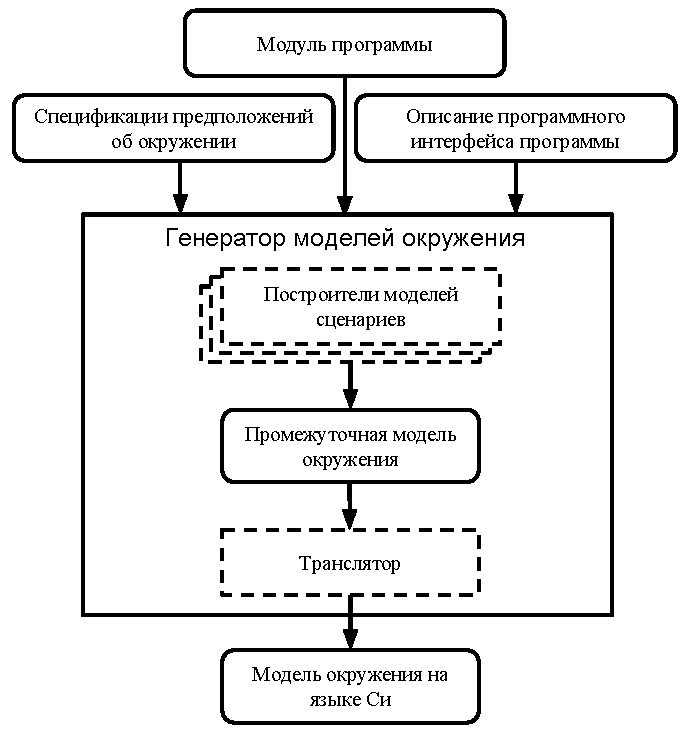
\includegraphics[scale=1.2]{generators}
\caption{Схема синтеза моделей окружения.}
\label{figure:em}
\end{figure}

Спецификации предположений об окружении содержат описания моделей сценариев взаимодействия на языке предметной области.
Построители выполняют подготовку моделей сценариев для промежуточной модели окружения на основе некоторого набора спецификаций предположений об окружении и описания программного интерфейса.
Предлагается использовать языки спецификации, расширяющие язык для задания промежуточной модели окружения, которым может быть либо язык Си расширениями для посылки и получения сигналов, либо специализированный язык предметной области.
Расширения должны учитывать особенности инструментов верификации, проверяемых требований, и верифицируемой программы.
Например, спецификация может представлять собой некоторый набор шаблонов моделей сценариев, на основе которых построитель может сгенерировать конкретные модели сценариев для промежуточной модели окружения. 
Для этого построитель определяет, какая часть программного интерфейса требует моделирования, определяя точки входа и неопределенные функции, а также другую необходимую информацию о программном интерфейсе.
Затем построитель использует те модели сценариев из спецификаций предположений об окружении, которые описывают вызов точек входа именно того модуля, для которого требуется подготовить модель окружения.

Предлагается использовать несколько построителей в зависимости от сложности и устройства верифицируемой программы.
Для крупных событийно-ориентированных программных систем на разработку построителей может требоваться значительное время.
Но универсальный алгоритм для данной задачи сформулировать трудно из-за широкого разнообразия программных систем и требований.

Рассмотрим пример работы простейшего построителя моделей сценариев для вызова функций по заданному пользователем списку имен.
Такой компонент выполняет следующие шаги:
\begin{enumerate}
    \item В качестве спецификации предположений об окружении пользователь передает список имен функций или шаблон, заданный при помощи регулярного выражения, и конфигурационные параметры, определяющие требуется ли вызывать функции в цикле.
    \item Построитель определяет на основе описания программного интерфейса конкретные функции, которые являются точками входа модуля программы и имена которых входят в список, заданный пользователем.
    Затем из описания программного интерфейса получаются сигнатуры точек входа.
    \item Для каждой функции выполняется генерация функции-обертки, помещаемой в тот файл, где определена точка входа. 
    Такая функция-обертка содержит инициализацию параметров с использованием вспомогательных функций для моделирования неопределенных значений, а также сам вызов целевой функции с данными параметрами.
    Обертка позволяет избежать ошибок, связанных с областью видимости типов, которые могут использоваться при задании сигнатуры аргументов точки входа, которую требуется вызвать.
    \item Построитель генерирует одну модель сценария для промежуточной модели окружения, которая вызывает точки входа. 
    Каждое действие модели сценария вызывает одну конкретную функцию-обертку.
    \item Отношение переходов, определяющее последовательность действий, зависит от конфигурационных параметров построителя.
    Если отношение переходов должно быть описано на языке программирования Си, тогда может использоваться оператор switch или цикл, в теле которого находится тот же оператор.
    Оператор switch в случайном порядке выполняет одно из действий --- вызов какой-либо функции-обертки.
    \item Все вспомогательные функции и модель сценария передаются транслятору.
\end{enumerate}

В некоторых случаях удобно вручную скорректировать или разработать модели сценариев для промежуточной модели окружения.
Такие модели сценариев необходимо иметь возможность передать в качестве входных данных генератору моделей окружения, чтобы они были добавлены в промежуточную модель для добавления к сгенерированным моделям сценариев, полученных построителями для определенных модулей, или для их замены.

Транслятор должен иметь ряд конфигурационных параметров, позволяющих настраивать вид модели окружения в зависимости от используемого инструмента верификации моделей программ или проверяемого требования.
На практике может возникать необходимость в следующих преобразованиях:
\begin{itemize}
    \item Выполнять трансляцию промежуточной модели окружения в последовательный или параллельный код на языке программирования Си. 
    При трансляции в последовательный код может требоваться подготовка модели окружения с разной степенью полноты с точки зрения всевозможных чередований событий из разных сценариев.
    \item Для задания параллельной модели окружения могут использоваться разные интерфейсы управления потоками или процессами.
    \item В модели окружения могут быть использованы разные наборы служебных функций.
\end{itemize}

В процессе своей работы транслятор выполняет следующие операции:
\begin{itemize}
    \item Объединяет полученные от построителей сценариев фрагменты промежуточной модели окружения на языке программирования Си, которые обозначались как $V_e, F_e, R_e, T_e$.
    \item Генерирует точку входа, которая вызывает служебную функцию инициализации модели требования.
    Затем в точке входа создаются потоки для сценариев, которые относятся к виду моделей потоков окружения.
    Для этого либо генерируется соответствующий код с созданием и ожиданием POSIX потоков, либо выполняется генерация последовательного кода с некоторым чередованием действий из разных сценариев.
    После завершения всех моделей сценариев в точке входа вызывается служебная функция завершения работы, определение которой находится в модели требования.
    \item Выполняет генерацию вспомогательного исходного кода для трансляции операций посылки и получения сигналов на язык программирования Си, например, в соответствие со схемой, предложенной при доказательстве теоремы об изоморфизме.
\end{itemize}

Модель окружения на языке программирования Си содержит набор файлов с исходным кодом, которые предлагается добавлять к модулю программы при помощи инструментации.
Данная операция выполняется на шаге компоновки верификационной задачи.

\section{Синтез моделей требований}

Для синтеза моделей требований предлагается использовать метод, предложенный ранее в работе~\cite{NovikovDis}.
Данный метод применялся в системе верификации LDV~Tools и показал возможность успешного применения на практике для проверки различных требований к драйверам операционной системы Linux~\cite{Zakharov2015, configurable:Trudy}.
Хотя в упомянутых работах метод применяется только для спецификации требований корректного использования интерфейса ядра в драйверах, он может быть использован и для других требований и программных систем.

Для формализации требования, согласно данному методу, требуется разработать контрактную спецификацию на аспектном расширении языка Си, называемую \textit{спецификацией требования}.
Спецификация содержит модели для функций и макрофункций программного интерфейса модулей программы, которые определены в окружении.
Спецификация позволяет свести задачу проверки требования к свойству корректности недостижимости ошибочного оператора.
Для некоторых требований, например, корректности работы с памятью, разрабатывать спецификацию нецелесообразно, так как модель требования будет чрезмерно сложной и вряд ли может быть проверена на практике инструментами верификации моделей программ.
В этом случае требование должно поддерживаться инструментом верификации в явном виде как проверка соответствующего свойства корректности.

Для генерации модели требования используется инструмент CIF для реализации подхода аспетно-ориентированного программирования, предложенного Е.~М.~Новиковым и апробированным при верификации драйверов ОС Linux в рамках системы верификации LDV~Tools~\cite{Novikov2013}.
Спецификация требования подается инструменту CIF вместе с исходным кодом модуля программы.
Инструмент выполняет препроцессирование исходного кода модуля и его инструментацию для синтеза модели требования на основе спецификации требования и добавления ее в исходный код модуля.

Спецификации предположений об окружении требований могут содержать определения одних и тех же функций.
Чтобы избежать конфликтов вводятся дополнительные служебные функции, которые определены в спецификации требования, но вызываются в модели окружения.
К таким служебным функциям относятся упомянутые ранее функции инициализации требования и функция завершения работы, которые соответствуют началу выполнения и завершению вызова точек входа модуля.
При вызове первой функции модель требования инициализирует начальное состояние,
а при вызове последней выполняет проверку условий, которые должны быть справедливы в момент завершения работы модуля или всех точек входа.
Например, при проверке требования корректной работы с некоторым счетчиком ссылок, модель требования инициализирует значение модели счетчика значением 0, а при вызове функции завершения работы проверяет, что все ссылки были успешно удалены и значение счетчика равно 0.

\section{Компоновка верификационных задач}
В качестве входных данных при компоновке верификационных задач выступают файлы с исходным кодом программы, файлы моделей окружения и требования, а также конфигурационные параметры, заданные пользователем.
В качестве результата компоновки из входных данных должна быть получена отдельная верификационная задача в формате, предложенном сообществом SV"~COMP.

Как ранее упоминалось, для получения исходного кода верификационной задачи может потребоваться инструментация исходного кода.
Для возможности применения данного метода модели должны быть сгенерированы в соответствующих форматах.
После или в процессе выполнения инструментации также следует препроцессировать исходный код всех файлов на языке программирования Си.
Некоторые инстрменты верификации моделей программ требуют, чтобы верификационная задача содержала только один файл.
В этом случае можно следует использовать инструменты для объединения файлов, например CIL~\cite{CIL}.

Для каждого требования следует подготовить соответствующую спецификацию свойства корректности и параметры в зависимости от инструмента верификации и его версии.
Комбинаций инструментов, версий и свойств корректности может быть достаточно много.
Поэтому может быть полезным ввести специальный формат с возможностью наследования наборов опций, чтобы сократить трудоемкость описания каждого набора конфигурационных параметров.

Последней частью верификационной задачи являются максимальные ограничения на вычислительные ресурсы: времени работы, процессорного времени, оперативной и дисковой памяти.
Набор ограничений позволяет также решать важную задачу воспроизводимости результатов.
Так как при использовании одной и той же аппаратуры важно иметь возможность воспроизвести результат и использовать полученные данные, например, для сравнения подходов к верификации или определения наиболее сложных для инструмента верификации верификационных задач с целью улучшить набор спецификаций.